\renewcommand{\thispart}{4 }
\renewcommand{\thispartname}{
    Learning Algorithms and\\ 
    Practical Issues in Neural Network Training}

\part{\thispartname}

% Cover page
\section{Outline}
%
% Cover page for giveb part
%

\title[\modulename - Part \thispart]
{
  {\bf 
   \modulename - 
   Part \thispart\\
  }
  \vspace{0.5cm}
  {\it 
   \color{yellow}
    \secname\\
  }
}
\author[C.Andreopoulos] {
  Professor Costas Andreopoulos\inst{1,2}, {\it FHEA}
}
\institute[Liverpool/STFC-RAL] {
   \inst{1} University of Liverpool, Department of Physics\\
   \vspace{0.3cm}
   {\it {\color{magenta} Lectures delivered at the University of Liverpool, 2024-25}}\\
   \vspace{0.2cm}
}
\date{\today}

\titlegraphic{
  
\includegraphics[height=30px]{images/logo/liverpool.png}
}

\begin{frame}[plain]
  \titlepage
\end{frame}




% Outline
%
% Table of contents to be displayed at the beginning of each part
%

\begin{frame}[t,allowframebreaks]{Outline for Part \thispart -}
  % Part \thispart (\secname) covers the following topics:\\
  % \vspace{0.5cm}
  \linespread{1.1}
  \setcounter{secnumdepth}{3}
  \setcounter{tocdepth}{3}
  % \tableofcontents[currentsection, hideothersubsections, sectionstyle=hide/hide]
  \tableofcontents[part=\thispart]
\end{frame}



% Learning objectives

\begin{frame}[t,allowframebreaks]{
    Learning objectives for Part \thispart -}

    In this part of our lecture series:
    \begin{itemize}
        \item A
        \item B
    \end{itemize}

\end{frame}

\section{Basics of gradient-based optimization}

\begin{frame}[t,allowframebreaks]{Gradient-based optimization -}


    Training a \gls{ml} model requires 
    some kind of \index{optimisation}\gls{optimisation}.
    \begin{itemize}
        \item however, training is not a {\bf pure} \gls{optimisation} problem, 
        as we will discuss later. (See section on `\Gls{generalisation}'. 
        \hyperlink{sec:Generalisation}{\beamerbutton{link}})
    \end{itemize}
    \vspace{0.2cm}

    Often, we try to achieve the \index{extremisation}\gls{extremisation} 
    (minimisation or maximisation) of an 
    \index{objective function}\gls{objective function} or 
    \index{criterion}\gls{criterion}.
    \begin{itemize}
        \item 
            When the \gls{objective function} is minimised, 
            it is often called the
            \index{cost function}\gls{cost function},
            \index{loss function}\gls{loss function}, or
            \index{error function}\gls{error function}$^(1)$.
    \end{itemize}
    \vspace{0.2cm}
    The values extremising a function, 
    are often denoted with a $^\star$ superscript.
    So, if $f(\vect{x}): \mathbb{R}^n \rightarrow \mathbb{R}$ 
    is an \gls{objective function}
    we may write:
    \begin{equation*}
        \vect{x}^{\star} = \mathrm{argmin} \; f(\vect{x})
        \;\;\;\;\; \textrm{or} \;\;\;\;\;
        \vect{x}^{\star} = \mathrm{argmax} \; f(\vect{x})
    \end{equation*}

    \vspace{0.1cm}
    \noindent\rule{4cm}{0.4pt}\\
    {\tiny
    (1) Note that some authors assign subtle differences in these terms,
    while others use them interchangeably.\\
    }
    
    \framebreak

    %
    %

    Suppose $y=f(x)$ is a function whose domain and range is $\mathbb{R}$.\\
    \vspace{0.2cm}

    The \index{derivative}\gls{derivative} of $f(x)$, is another function 
    denoted as $f^\prime(x)$ or $df(x)/dx$.\\
    \vspace{0.3cm}
    
    The function $f^\prime(x)$:
    \begin{itemize}
        \item
        gives the {\bf slope of $f(x)$ at $x$} or, in other words,
        \item
        describes how to         
        scale a small change in the input $x$
        to compute a first-order approximation of the function $f$ at the new point:
        \begin{equation}
          f(x+\epsilon) \approx f(x) + \epsilon \; f^\prime(x)  
          \label{eq:deriv_1}
       \end{equation}\\
    \end{itemize}
    If $f(\vect{x})$
    is a scalar function of $n$ parameters,  
    the \index{gradient}\gls{gradient} $\nabla_{\vect{x}} f(\vect{x})$:
    \begin{equation}
        \nabla_{\vect{x}} f(\vect{x}) = 
        \Big( 
            \frac{\partial f(\vect{x})}{\partial x_1},
            \frac{\partial f(\vect{x})}{\partial x_2},
            \cdots ,
            \frac{\partial f(\vect{x})}{\partial x_n}
        \Big)
        \label{eq:gradient_1}
     \end{equation}\\
     generalises the concept of the \gls{derivative} in $n$-dimensional spaces.

    \framebreak

    %
    %

    {\bf The \index{gradient}\gls{gradient} $\nabla_{\vect{x}} f(\vect{x})$ 
    is useful for the 
    \index{extremisation}\gls{extremisation} of $f(\vect{x})$.}\\
    \vspace{0.2cm}
    \begin{itemize}
        \item
            It specifies how to make a small step in the space of $\vect{x}$, 
            in order to make a small improvement in $f(\vect{x})$ 
            in the desired direction.\\
            \vspace{0.1cm}
        \item
            Starting from a point $\vect{x}$, a calculation of 
            the \index{gradient}\gls{gradient} allows one to
            propose a new point $\vect{x}^\prime$ 
            on the path towards the function minimum$^{(1)}$:
            \begin{equation}
                \vect{x} \rightarrow \vect{x}^\prime = 
                    \vect{x} - \alpha \nabla_{\vect{x}} f(\vect{x})
                \label{eq:grad_descent_1}
            \end{equation}\\
            where $\alpha$ is a \index{hyperparameter}\gls{hyperparameter}
            controlling the \index{learning rate}\gls{learning rate}.
    \end{itemize}

    \vspace{0.1cm}

    This iterative \index{optimisation}\gls{optimisation} 
    technique is known as 
    \index{gradient}\index{gradient descent}{\bf \gls{gradient descent}}.
    \begin{itemize}
      \small
      \item The method is attributed to L.A. Cauchy (1847)
       \cite{Cauchy:GradientDescent}, who used it to solve systems of
       simultaneous equations that determine the orbits of stars.
    \end{itemize}

    \vspace{0.1cm}
    \noindent\rule{4cm}{0.4pt}\\
    {\tiny
    (1) Similarly, if we seek to maximise $f(\vect{x})$ 
    we move up the slope
    $\displaystyle \vect{x} \rightarrow \vect{x}^\prime =
      \vect{x} {\color{cadmiumred}+} \alpha \nabla_{\vect{x}} f(\vect{x})$.\\
    }

    \framebreak

    %
    %

    \vspace{-1.0cm}

    \begin{center}
        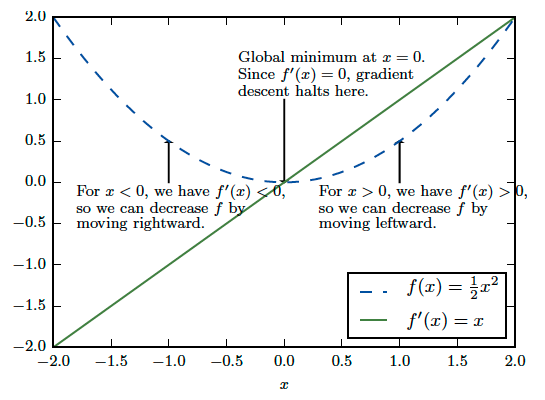
\includegraphics[width=0.80\textwidth]
            {./images/grad_descent/goodfellow17_grad_descent_1d.png}\\
        {\tiny 
            Simple illustration of the method of
            \index{gradient}\index{gradient descent}{\bf \gls{gradient descent}}.
            \color{col:attribution} 
            Schematic reproduced from p. 80 of \cite{Goodfellow:2017MITDL}.\\
        }
    \end{center}        

    \framebreak

    %
    %

    The \index{gradient}\index{gradient descent}\gls{gradient descent} method
    readily generalizes in multiple dimensions.\\


    \begin{columns}
        \begin{column}{0.80\textwidth}
            \begin{center}
                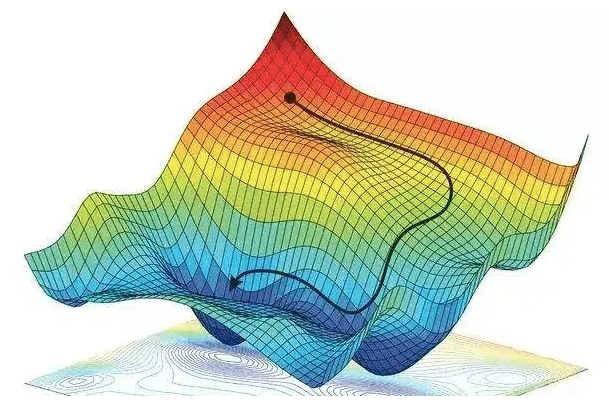
\includegraphics[width=0.99\textwidth]
                    {./images/grad_descent/guliyev20_grad_descent_2d.png}\\
                {\tiny 
                    Simple illustration of the method of
                    \index{gradient}\index{gradient descent}{\bf \gls{gradient descent}}.
                    \color{col:attribution} 
                    Schematic reproduced from \cite{Medium:GradDescentOptLinReg}.\\
                }
            \end{center}                    
        \end{column}
        \begin{column}{0.20\textwidth}
        {\scriptsize
            The method has several weaknesses when applied to
            optimization problems in multiple dimensions.\\
            \vspace{0.2cm}
            Later in this lecture, 
            we will discuss these weaknesses and 
            improved algorithms.\\
        
        }    
        \end{column}
    \end{columns}

    \framebreak

    %
    %

    There are various types of 
    \index{gradient}\index{gradient descent}{\bf \gls{gradient descent}}
    algorithms:\\
    \begin{itemize}
        \item   
            \index{batch gradient descent}
            \Gls{batch gradient descent}\\
            \begin{itemize}
                \item
                    Updates the model parameters 
                    after an iteration over all examples in the training set
                    (defining a training \index{epoch}\gls{epoch}).
            \end{itemize}
        \item 
            \index{mini batch gradient descent}
            \Gls{mini batch gradient descent}\\
            \begin{itemize}
                \item   
                    Separates the training set into small batches,
                    and updates the model parameters after an iteration
                    over all examples of each batch.
            \end{itemize}
        \item 
            \index{stochastic gradient descent}
            \Gls{stochastic gradient descent}\\
            \begin{itemize}
                \item   
                    Updates the model parameters after evaluating each
                    single example in the training set.\\
            \end{itemize}
    \end{itemize}

    \framebreak

    %
    %

    \vspace{-0.5cm}
    As we have seen, 
    \index{gradient}\index{gradient descent}\gls{gradient descent} 
    proposes a step (Eq.~\ref{eq:grad_descent_1}) 
    from $\vect{x}$ to $\vect{x}^\prime$:\\
    \vspace{-0.2cm}
    \begin{equation*}
        \vect{x} \rightarrow \vect{x}^\prime = 
            \vect{x} - \alpha \nabla_{\vect{x}} f(\vect{x})
    \end{equation*}\\
    \vspace{-0.1cm}
    The method is {\bf sensitive to the value of the 
    \index{learning rate}\gls{learning rate}, $\alpha$}.\\
    \begin{itemize}
        \small
        \item 
        If too large, the algorithm can 
        overshoot and step past the minimum.
        \item 
        If too small, the algorithm can become 
        too inefficient.
    \end{itemize}
    \begin{center}
        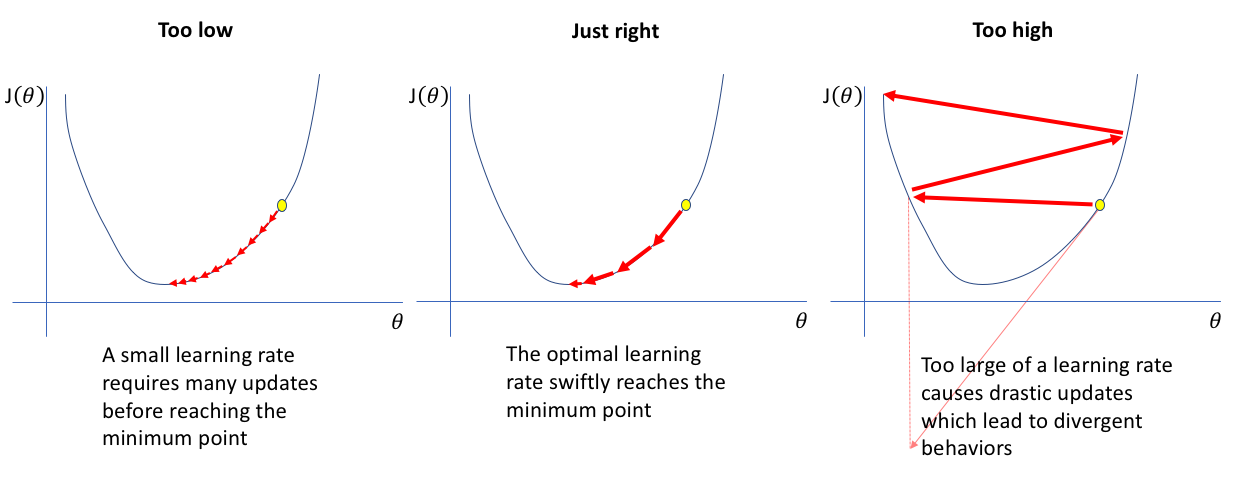
\includegraphics[width=0.88\textwidth]
            {./images/grad_descent/atu22_learning_rate_1.png}\\
        {\tiny 
            \color{col:attribution} 
            Schematic reproduced from \cite{Medium:GradDescent}.\\
        }
    \end{center}                    

    \framebreak

    %
    %

    There are several ways to choose the value of 
    the \index{learning rate}\gls{learning rate}, $\alpha$.\\
    \vspace{0.2cm}
    For example, we can:
    \begin{itemize}
        \item 
          set $\alpha$ to a small constant value,
        \item 
          solve for the value of $\alpha$ that makes the 
          directional derivative $\frac{\partial f(\vect{x})}{\partial \vect{n}}^{(1)}$ 
          vanish, i.e. move along $-\nabla_{\vect{x}} f(\vect{x})$
          till $f$ no longer descents, or
        \item 
          evaluate $f\big(\vect{x} - \alpha \nabla_{\vect{x}} f(\vect{x})\big)$
          for a range of $\alpha$ values, and  pick the one that leads to the smallest
          value of $f$ ({\bf line search} strategy).
    \end{itemize}
    \vspace{0.2cm}
    The choice impacts the {\bf efficient convergence} of the optimization.\\
    %\vspace{0.1cm}
    \noindent\rule{4cm}{0.4pt}\\
    \vspace{0.1cm}
    {\tiny
    (1) The directional derivative, 
    $\frac{\partial f(\vect{x})}{\partial \vect{n}}$,
    is the derivative of $f(\vect{x})$ in the direction of $\vect{\hat{n}}$. 
    It should not be confused with the gradient 
    $\nabla_{\vect{x}} f(\vect{x})$ though,
    clearly, they are connected: 
    $\frac{\partial f(\vect{x})}{\partial \vect{n}} = 
     \vect{n} \cdot \nabla_{\vect{x}} f(\vect{x})$.\\
    }


    \framebreak

    %
    %

    Points where the 
    \index{derivative}\gls{derivative} $f^\prime(x)$ 
    takes the value of 0  are known as 
    \index{critical point}\glspl{critical point} or 
    \index{stationary point}\glspl{stationary point}.\\

    \vspace{0.2cm}

    \begin{columns}
        \begin{column}{0.32\textwidth}
            These points are either: 
            \begin{itemize}
              \item \index{local minimum}\glspl{local minimum}, 
              \item \index{local maximum}\glspl{local maximum}, or
              \item \index{saddle point}\glspl{saddle point}.\\        
            \end{itemize}
            \end{column}
        \begin{column}{0.68\textwidth}

            \begin{center}
                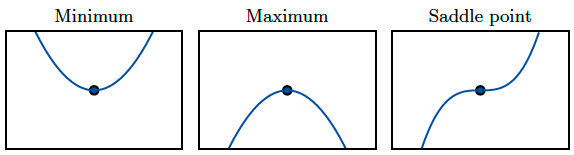
\includegraphics[width=0.80\textwidth]
                    {./images/grad_descent/goodfellow17_min_max_saddle_1d.png}\\
                {\tiny 
                    \color{col:attribution} 
                    Schematic reproduced from p. 81 of \cite{Goodfellow:2017MITDL}.\\
                }

                \vspace{0.6cm}

                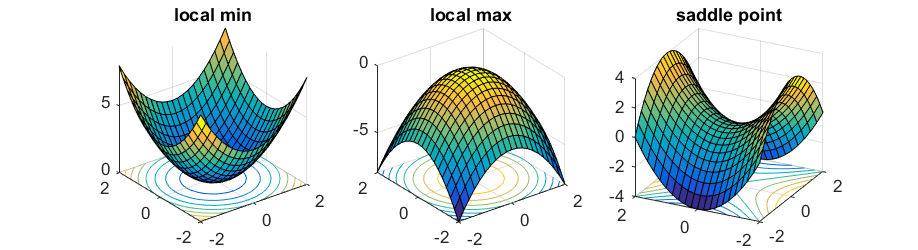
\includegraphics[width=0.99\textwidth]
                    {./images/grad_descent/ge16_min_max_saddle_2d.png}\\
                {\tiny 
                    \color{col:attribution} 
                    Schematic reproduced from \cite{OffConvex:EscapingSaddlePoints}.\\
                }
            \end{center}        
        
        \end{column}
    \end{columns}

\end{frame}



\section{Beyond the gradient}
\subsection{The Jacobian matrix}

\begin{frame}[t,allowframebreaks]{
    Beyond the gradient: The Jacobian matrix -}

    Suppose $f$ is a function 
    whose input \underline{and} output are vectors.\\
    \vspace{0.2cm}

    If $f$: $\mathbb{R}^m \rightarrow \mathbb{R}^n$,
    all the first-order partial derivatives of $f$ can be written 
    as a matrix $\vect{J}$ $\in \mathbb{R}^{m \times n}$
    defined such that:

    \begin{equation}
        J_{ij} = 
        \frac{\partial f_{i}(\vect{x})}{\partial x_j}
        \label{eq:jacobian_1}
    \end{equation}\\

    Therefore: 
    \begin{equation}
        \vect{J} = 
        \left(
            \begin{array}{ccc}
            \frac{\partial \vect{f}(\vect{x})}{\partial x_1} & 
            \cdots & 
            \frac{\partial \vect{f}(\vect{x})}{\partial x_n} \\ 
            \end{array}
        \right) =
        \left(
            \begin{array}{c}
            \nabla_{\vect{x}}^T f_{1}(\vect{x}) \\
            \vdots \\
            \nabla_{\vect{x}}^T f_{m}(\vect{x}) \\
            \end{array}
        \right) =
        \left(
            \begin{array}{ccc}
            \frac{\partial f_{1}(\vect{x})}{\partial x_1} & 
            \cdots & 
            \frac{\partial f_{1}(\vect{x})}{\partial x_n} \\ 
            \vdots &
            \ddots & 
            \vdots \\
            \frac{\partial f_{m}(\vect{x})}{\partial x_1} & 
            \cdots & 
            \frac{\partial f_{m}(\vect{x})}{\partial x_n} \\ 
            \end{array}
        \right)
        \label{eq:jacobian_2}
    \end{equation}\\

    \vspace{0.2cm}

    This matrix of derivatives is known as a
    \index{Jacobian matrix}\Gls{Jacobian matrix}.
    It has {\bf a range of applications} in several fields.\\

    \framebreak

    %
    %

    The Jacobian can be used to approximate a nonlinear 
    function with a linear one:
    \begin{equation}
        f(\vect{x}^\prime) \approx 
        f(\vect{x}) + \vect{J}(\vect{x}) \cdot (\vect{x}^\prime - \vect{x})   
        \label{eq:jacobian_linearization_1}
    \end{equation}\\
    is the generalization of Eq.~\ref{eq:deriv_1}
    for a function $f$: $\mathbb{R}^m \rightarrow \mathbb{R}^n$.

    %  \begin{center}
    %     \includegraphics[width=0.75\textwidth]
    %         {./images/grad_descent/jacobian.png}\\
    %     {\tiny 
    %         Simple illustration of the gradient descent technique.
    %         \color{col:attribution} 
    %         Schematic reproduced from p. 80 of \cite{Goodfellow:2017MITDL}.\\
    %     }
    %  \end{center}        

\end{frame}

\subsection{The Hessian matrix}


\begin{frame}[t,allowframebreaks]{
    Beyond the gradient: The Hessian matrix -}

    Often, we are interested to know {\bf how the 
    \underline{first derivative} of a 
    function will change as we vary the input} of the function.\\
    \begin{itemize}
        \item
        Naturally, this information is described by the 
        \underline{second derivative} of the function 
        (ie. the derivative of the derivative).\\
    \end{itemize}

    \vspace{0.2cm}

    The second derivative of a function is {\bf a measure of its curvature}.\\

    \begin{columns}
        \begin{column}{0.42\textwidth}
        
            The curvature determines

        \end{column}
        \begin{column}{0.58\textwidth}

            \begin{center}
                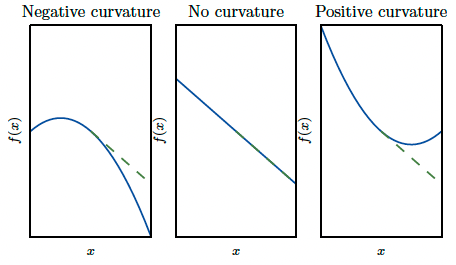
\includegraphics[width=1.00\textwidth]
                    {./images/grad_descent/goodfellow17_curvature_1d.png}\\
                {\tiny 
                    \color{col:attribution} 
                    Schematic reproduced from p. 84 of \cite{Goodfellow:2017MITDL}.\\
                }
            \end{center}        
        
        \end{column}
    \end{columns}

    \framebreak

    %
    %
   
    Suppose we have a function 
    $f(\vect{x})$: $\mathbb{R}^m \rightarrow \mathbb{R}$.
    The derivative wrt $x_i$ of the derivative of $f$ wrt to $x_j$ 
    is denoted by $\displaystyle \partial^2 f(\vect{x}) / \partial x_i \partial x_j$.\\        
    \vspace{0.1cm}

    These partial derivatives form the \gls{Hessian matrix} 
    $\vect{H}^{(f)}(\vect{x})$ with elements:
    \begin{equation}
        H^{(f)}_{ij}(\vect{x}) = 
        \frac{\partial^2 f(\vect{x})}{\partial x_i \partial x_j}
        \label{eq:hessian_1}
    \end{equation}\\
    
    Therefore:\\
    \vspace{-0.2cm}
    \begin{equation}
        \vect{H}^{(f)}(\vect{x}) = 
        % \left(
        %     \begin{array}{ccc}
        %         \frac{\partial \vect{f}(\vect{x})}{\partial x_1} & 
        %         \cdots & 
        %         \frac{\partial \vect{f}(\vect{x})}{\partial x_n} \\ 
        %     \end{array}
        % \right) =
        % \left(
        %     \begin{array}{c}
        %         \nabla_{\vect{x}}^T f_{1}(\vect{x}) \\
        %         \vdots \\
        %         \nabla_{\vect{x}}^T f_{m}(\vect{x}) \\
        %     \end{array}
        % \right) =
        \left(
            \begin{array}{cccc}
                \frac{\partial^2 f(\vect{x})}{\partial x_1^2} & 
                \frac{\partial^2 f(\vect{x})}{\partial x_1 \partial x_2} &
                \cdots & 
                \frac{\partial^2 f(\vect{x})}{\partial x_1 \partial x_m} \\ 
                \frac{\partial^2 f(\vect{x})}{\partial x_2 \partial x_1} & 
                \frac{\partial^2 f(\vect{x})}{\partial x_2^2} &
                \cdots & 
                \frac{\partial^2 f(\vect{x})}{\partial x_2 \partial x_m} \\ 
                \vdots &
                \vdots &
                \ddots & 
                \vdots \\
                \frac{\partial^2 f(\vect{x})}{\partial x_m \partial x_1} & 
                \frac{\partial^2 f(\vect{x})}{\partial x_m \partial x_2} & 
                \cdots & 
                \frac{\partial^2 f(\vect{x})}{\partial x_m^2} \\ 
            \end{array}
        \right)
        \label{eq:hessian_2}
    \end{equation}\\
    
    \vspace{0.25cm}

    \index{Hessian matrix}\index{Jacobian matrix}
    Note that {\bf the \gls{Hessian} is the \gls{Jacobian} of the gradient}.

    \framebreak

    %
    %

    \begin{itemize}
        \item 
        Anywhere the second-order partial derivatives are continuous,
        the \gls{Hessian matrix} is {\bf symmetric}:
        \begin{equation}
            H^{(f)}_{ij}(\vect{x}) = 
              \frac{\partial^2 f(\vect{x})}{\partial x_i \partial x_j} =
              \frac{\partial^2 f(\vect{x})}{\partial x_j \partial x_i} =
              H^{(f)}_{ji}(\vect{x}) 
            \label{eq:hessian_symmetric_1}
         \end{equation}\\
         \begin{equation}
              \vect{H}^{(f)}(\vect{x}) = \Big( \vect{H}^{(f)}(\vect{x}) \Big)^T
            \label{eq:hessian_symmetric_2}
         \end{equation}\\
    
        \item 
        Because $\vect{H}^{(f)}(\vect{x})$ is real and symmetric,
        it can be decomposed into a set of real 
        \index{eigenvalue}\glspl{eigenvalue} $\lambda_{i}$
        and an orthogonal basis of 
        \index{eigenvector}\glspl{eigenvector} $\vect{\hat{e}}_i$.
        $\vect{H}^{(f)}(\vect{x})$ is {\bf diagonalizable} and
        there exist a matrix $\vect{O}$ such that:
        \begin{equation}
            \vect{H}^{(f)}(\vect{x}) = 
            \vect{O}
            \left(
                \begin{array}{ccc}
                    \lambda_1 &        & \\
                              & \ddots & \\
                              &        & \lambda_m \\                              
                \end{array}
            \right)
            \vect{O}^{-1}
          \label{eq:hessian_diag_1}
       \end{equation}\\
    \end{itemize}

    \framebreak

    %
    %

    \begin{itemize}
        \item 
        The second derivative in a particular direction
        expressed by a unit vector $\vect{\hat{u}}$ is given by
        $\displaystyle \vect{\hat{u}}^T \cdot \vect{H}^{(f)}(\vect{x}) \cdot \vect{\hat{u}}$.
        \begin{itemize}
            \item If $\vect{\hat{u}}$ is one of the 
            \index{eigenvector}\glspl{eigenvector}, $\vect{\hat{e}}_i$,
            {\bf the corresponding 
            \index{eigenvalue}\gls{eigenvalue} gives the second-order 
            derivative in that direction}.
            \item In all other directions, the directional 
            {\bf second-order derivative is 
            a weighted average of all \glspl{eigenvalue} $\lambda_{i}$}.
            \begin{itemize}
                \item All weights are between 0 and 1.
                \item Eigenvalues with larger weight correspond to \glspl{eigenvector}
                $\vect{\hat{e}}_i$ that are closer to the direction of $\vect{\hat{u}}$.
            \end{itemize}
            \item The minimum (maximum) \gls{eigenvalue} determined the minimum (maximum)
            directional second-order derivative.
        \end{itemize}
    
    \end{itemize}

    \framebreak

    %
    %

    Using a second-order \index{Taylor series}\gls{Taylor series}, we can approximate 
    the value of the function $f$ at $\vect{x}^\prime$, 
    a small distance away from $\vect{x}$:
    \vspace{-0.1cm}
    \begin{equation}
        f(\vect{x}^\prime) \approx 
          f(\vect{x}) + 
          (\vect{x}^\prime - \vect{x})^T \cdot \nabla_{\vect{x}}f(\vect{x}) +
          \frac{1}{2} (\vect{x}^\prime - \vect{x})^T \cdot 
            \vect{H}^{(f)}(\vect{x}) \cdot (\vect{x}^\prime - \vect{x})
        \label{eq:hessian_taylor_1}
    \end{equation}

    If $\alpha$ is the \index{learning rate}\gls{learning rate}, 
    the gradient-based optimization procedure moves from point $\vect{x}$ 
    to the point $\vect{x}^\prime$ given by Eq.~\ref{eq:grad_descent_1}
    ($\displaystyle \vect{x}^\prime = \vect{x} - \alpha \nabla_{\vect{x}}f(\vect{x})$).\\
    \vspace{0.2cm}

    Substituting Eq.~\ref{eq:grad_descent_1} into Eq.~\ref{eq:hessian_taylor_1}, 
    we obtain:
    \vspace{-0.1cm}
    \begin{equation}
        f(\vect{x}^\prime) \approx 
        f(\vect{x}) 
        {\color{cadmiumgreen}
          - \alpha 
           \nabla_{\vect{x}}^{T}f(\vect{x}) \cdot 
           \nabla_{\vect{x}}f(\vect{x})      
        } 
        {\color{cadmiumred}      
           + \frac{1}{2} \alpha^2 
           \nabla_{\vect{x}}^{T}f(\vect{x}) \cdot 
           \vect{H}^{(f)}(\vect{x}) \cdot 
           \nabla_{\vect{x}}f(\vect{x})
        } 
        \label{eq:hessian_taylor_2}
    \end{equation}

    In Eq.~\ref{eq:hessian_taylor_2}, we recognize three terms describing:\\
    \begin{itemize}
        \item the original value of $f$,
        \item the {\color{cadmiumgreen}expected improvement due to the gradient of $f$}, and
        \item a {\color{cadmiumred}correction that accounts for the curvature of $f$}.
    \end{itemize}

    \framebreak

    %
    %

    The last term in Eq.~\ref{eq:hessian_taylor_2} is a
    {\color{cadmiumred}correction accounting for the curvature of $f$}.\\
    \vspace{-0.5cm}
    \begin{equation*}
        f(\vect{x}^\prime) \approx 
        f(\vect{x}) 
        {\color{cadmiumgreen}
          - \alpha 
           \nabla_{\vect{x}}^{T}f(\vect{x}) \cdot 
           \nabla_{\vect{x}}f(\vect{x})      
        } 
        {\color{cadmiumred}    
         \overbrace{  
           + \frac{1}{2} \alpha^2 
           \nabla_{\vect{x}}^{T}f(\vect{x}) \cdot 
           \vect{H}^{(f)}(\vect{x}) \cdot 
           \nabla_{\vect{x}}f(\vect{x})
         }^\text{$\delta_{curv}$}
        } 
    \end{equation*}

    Note that:
    \begin{itemize}
        \item 
        When $\delta_{curv} \le 0$, Eq.~\ref{eq:hessian_taylor_2} predicts that
        $f(\vect{x})$ will keep on decreasing for any value of $\alpha$,
        but the expansion will not remain accurate 
        for large $\alpha$.
        The optimal step size is found by trial and error.\\
        \item 
        When $\delta_{curv} > 0$, the optimal step size can be found by minimizing the 
        right-hand side of Eq.~\ref{eq:hessian_taylor_2} that is quadratic in $\alpha$:
        \begin{equation}
            \alpha_{opt} = 
            \frac{
                \nabla_{\vect{x}}^{T}f(\vect{x}) \cdot 
                \nabla_{\vect{x}}f(\vect{x})
            }{
                \nabla_{\vect{x}}^{T}f(\vect{x}) \cdot
                \vect{H}^{(f)}(\vect{x}) \cdot 
                \nabla_{\vect{x}}f(\vect{x})
            }
            \label{eq:taylor_optimum_step_1}     
        \end{equation}
        \item 
        If $\delta_{curv}$ is too large, 
        the \index{gradient descent}\gls{gradient descent} 
        step can move uphill!
    \end{itemize}

    \framebreak

    %
    %

    Using the 2$^{nd}$ derivative, $f^{\prime \prime}(x)$, we can determine whether a
    \index{critical point}\gls{critical point} (where $f^{\prime}(x)=0$) is a
    \index{local maximum}\gls{local maximum}, a
    \index{local minimum}\gls{local minimum}, or a
    \index{saddle point}\gls{saddle point}.\\        
    \vspace{-0.1cm}

    \begin{columns}
        \begin{column}{0.60\textwidth}        
            \begin{center}
                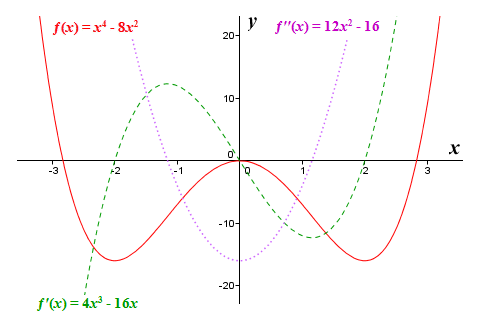
\includegraphics[width=1.00\textwidth]
                    {./images/grad_descent/techuk_second_derivative_test_1.png}\\
                {\tiny 
                    \color{col:attribution} 
                    Schematic reproduced from \cite{TechUK:2ndDerivativeTest}.\\
                }
            \end{center}        
        \end{column}
        \begin{column}{0.40\textwidth}
            \begin{itemize}
                \item If $f^{\prime \prime}(x) > 0$
            \end{itemize}
                
        \end{column}
    \end{columns}

    \vspace{0.1cm}
    In multiple dimensions, 
    we need to examine all the 2$^{nd}$-order derivatives
    of the function. The \index{Hessian matrix}\gls{Hessian matrix} supports this task.\\

    \framebreak

    %
    %

    The 2$^{nd}$ derivative test can be generalized in multiple dimensions
    using the \index{eigendecomposition}\gls{eigendecomposition} 
    of the \index{Hessian matrix}\gls{Hessian matrix}.\\
    \vspace{0.3cm}
    A \index{critical point}\gls{critical point},
    where $\nabla_{\vect{x}} f(\vect{x})=0$, is:
    \begin{itemize}
        \item 
        a \index{local minimum}\gls{local minimum}, 
        if the \gls{Hessian matrix} is 
        \index{positive definite}{\bf \gls{positive definite}}\\ 
        (i.e. all its \index{eigenvalue}\glspl{eigenvalue} are positive)
        \item 
        a \index{local maximum}\gls{local maximum}, 
        if the \gls{Hessian matrix} is 
        \index{negative definite}{\bf \gls{negative definite}}\\ 
        (i.e. all its \glspl{eigenvalue} are negative)
        \item 
        a \index{saddle point}\gls{saddle point}, 
        if at least one \gls{eigenvalue} is positive 
        and at least another one is negative.
    \end{itemize}

    \vspace{0.3cm}

    In multiple dimensions, the 2$^{nd}$ derivative 
    test can be {\bf inconclusive} 
    if at least one \gls{eigenvalue} is zero and 
    all nonzero \glspl{eigenvalue} have the same sign.

    \framebreak

    %
    %

    \begin{columns}
        \begin{column}{0.70\textwidth}        
            \begin{center}
                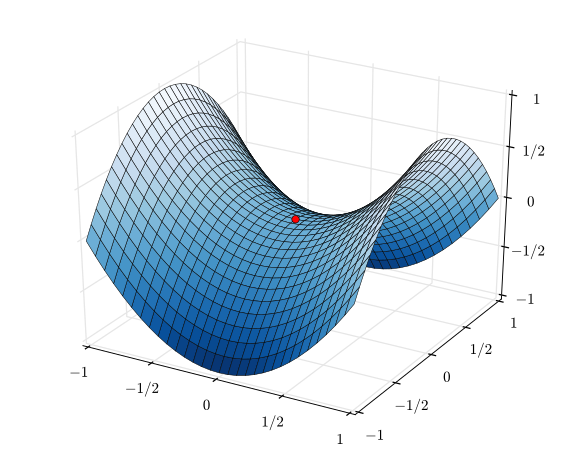
\includegraphics[width=1.00\textwidth]
                    {./images/grad_descent/wikipedia_saddle_point.png}\\
                {\tiny 
                    \vspace{0.2cm}
                    A saddle point.\\
                    \color{col:attribution} 
                    Schematic reproduced from \cite{Wikipedia:SaddlePoint}.\\
                }
            \end{center}        
        \end{column}
        \begin{column}{0.30\textwidth}
            {\small
            In multiple dimensions, it is not necessary to have a zero
            2$^{nd}$ derivative to get a \index{saddle point}\gls{saddle point}.\\
            \vspace{0.3cm}.
            At a \gls{saddle point},
            a function has both positive and negative curvature.\\
            \vspace{0.3cm}
            On a cross-section of the plot on the left,
            the point is a \index{local minimum}\gls{local minimum},
            whereas on another cross-section it is
            a \index{local maximum}\gls{local maximum}.\\
            }
        \end{column}
    \end{columns}

\end{frame}



\begin{frame}[t,allowframebreaks]{Hessian condition number -}

    The \index{Hessian condition number}\gls{Hessian condition number}, 
    $\kappa$, is defined as:
    \begin{equation}
        \kappa \Bigl[ \vect{H}^{(f)}(\vect{x}) \Bigr] 
          = \frac{\lambda_{max}}{\lambda_{min}}
        \label{eq:hessian_condition_number_1}
    \end{equation}

    where $\lambda_{max}$ is the largest 
    \index{eigenvalue}\gls{eigenvalue} 
    of the \index{Hessian matrix}\gls{Hessian matrix} 
    $\vect{H}^{(f)}(\vect{x})$, and  $\lambda_{min}$ 
    is the smallest one.\\
    
    \vspace{0.2cm}

    The \gls{condition number} characterises 
    the curvature of $f$ at point $\vect{x}$, and measures
    how much the 2$^{nd}$-order derivatives differ from each other.

    \begin{itemize}
        \item
        A value of $\kappa$ close to 1 (i.e. all the \glspl{eigenvalue} are similar in size), 
        suggests that the surface of the function 
        is relatively smooth and it does not vary very differently in different directions.
        \item
        If $\kappa >> 1$, the surface of the function is highly curved
        and changes very differently in different directions.
        \item
        If $\kappa << 1$,
    \end{itemize}

    It is a measure of how {\em well-conditioned} or 
    {\em ill-conditioned} is the curvature of a function at a given point.
    For ill-conditioned problems convergence of the 
    \index{gradient descent}\gls{gradient descent} method can be slow\\


\end{frame}

\begin{frame}[t,allowframebreaks]{Ill conditioning -}

\end{frame}



\section{Difficulties in convergence}

\subsection{Vanishing and exploding gradient problems}

\begin{frame}[t,allowframebreaks]{
    Vanishing and exploding gradients -}

    Self-evidently, the method of 
    \index{gradient}\index{gradient descent}\gls{gradient descent}
    requires {\em useful} \index{gradient}\glspl{gradient}.\\
    \vspace{0.2cm}
    Deep neural networks often have 
    training issues associated with either 
    {\bf vanishing} or {\bf exploding} \glspl{gradient}.\\
    \vspace{0.1cm}
    \begin{itemize}
        \small
        \item 
        If the \gls{gradient} is too small, 
        it becomes ineffective or impossible 
        to obtain updates for the network weights,
        especially for the initial layers.
        \item 
        If the \gls{gradient} is too large,
        weight updates become very large destabilising
        the learning process or halting it through numerical overflows. 
    \end{itemize}
    In both cases, {\bf networks becomes unable to learn}.\\
    \vspace{0.2cm}
    Issues arise from the way \glspl{derivative} in
    earlier and later layers are linked.\\
    \begin{itemize}
        \small
        \item
        In \index{back propagation}\gls{back propagation},
        the \glspl{derivative} of the network are found by moving 
        layer by layer, from the final back to the initial one.\\
        \item 
        Using the {\bf chain rule}, \glspl{derivative} of each layer
        are {\bf multiplied across the depth of the network}.
        \item 
        This product of \glspl{derivative} can become
        {\bf problematic for deep networks}, when the product
        includes a large number of terms.
    \end{itemize}

    \framebreak

    %
    %

    Consider a {\bf deep network} with $m$+1 layers, 
    incl. the input/output ones.\\
    Further assume that there is a {\bf single node per layer}.\\
    \vspace{0.2cm}
    Let $x$ (or $y_0$) be the input, $o$ (or $y_m$) the output, and
    $y_{1}, y_{2},...,y_{m-1}$ the output of each of the $m$+1 hidden layers.\\
    \vspace{0.2cm}
    Each computational layer $k$, applies the sigmoid function
    \begin{equation}
        \sigma(z_{k}) = \frac{1}{1+e^{-z_{k}}}
     \end{equation} 
    on its input $z_k$, which is computed as $z_k = w_{k}y_{k-1}+b_{k}$.

    
\begin{center}
    \begin{tikzpicture}[scale=0.8]
   
       %\draw[help lines] (0,0) grid (15,3);
       
       \node[ann_input_node] (x)    
         at ( 1.0, 1.5) {\Large $x$};
       \node[ann_processing_node] (h1)   
         at ( 3.5, 1.5) {\Large $\sigma$};
       \node[ann_processing_node] (h2)   
         at ( 6.0, 1.5) {\Large $\sigma$};
       \node[ann_processing_node_rep] (hi)   
         at ( 8.5, 1.5) {\Large $...$};
       \node[ann_processing_node] (hm_1) 
         at (11.5, 1.5) {\Large $\sigma$};
       \node[ann_processing_node] (o)    
         at (14.5, 1.5) {\Large $\sigma$};       

       \drawgraphlinebigarrow (x.east)       
         to[left =0] 
           node[above,midway,xshift=0.4cm,yshift=0.3cm]
             {$z_1$}
           node[below,midway,xshift=0.0cm,yshift=-0.2cm]
             {$w_1,b_1$}
         (h1.west) ;

       \drawgraphlinebigarrow (h1.east)       
         to[left =0] 
           node[above,midway,xshift=-0.4cm,yshift=0.3cm]
             {$y_1$}
           node[above,midway,xshift=0.4cm,yshift=0.3cm]
             {$z_2$}
           node[below,midway,xshift=0.0cm,yshift=-0.2cm]
             {$w_2,b_2$}
         (h2.west) ;

       \drawgraphlinebigarrow (h2.east)       
         to[left =0] 
           node[above,midway,xshift=-0.4cm,yshift=0.3cm]
             {$y_2$}
           node[below,midway,xshift=0.0cm,yshift=-0.2cm]
             {$w_3,b_3$}
         (hi.west) ;

       \drawgraphlinebigarrow (hi.east)       
         to[left =0] 
           node[above,midway,xshift=0.3cm,yshift=0.3cm]
             {$z_{m-1}$}
           node[below,midway,xshift=-0.1cm,yshift=-0.2cm]
             {$w_{m-1},b_{m-1}$}
         (hm_1.west) ;

       \drawgraphlinebigarrow (hm_1.east)       
         to[left =0] 
           node[above,midway,xshift=-0.4cm,yshift=0.3cm]
             {$y_{m-1}$}
           node[above,midway,xshift=0.5cm,yshift=0.3cm]
             {$z_{m}$}
           node[below,midway,xshift=0.0cm,yshift=-0.2cm]
             {$w_{m},b_{m}$}
         (o.west) ;

       \drawgraphlinebigarrow (o.east)       
         to[left =0] 
           node[above,midway,xshift=-0.1cm,yshift=0.3cm]
             {$o$}
         (15.8,1.5) ;
         
    \end{tikzpicture}
\end{center}


    \framebreak

    %
    %

    \vspace{-1.0cm}

    Therefore, the network evaluates the following expressions:
    \begin{equation}
       o = \sigma(z_m) = \sigma(w_{m} y_{m-1} + b_{m}) 
    \end{equation}
    \begin{equation}
        y_{m-1} = \sigma(z_{m-1}) = \sigma(w_{m-1} y_{m-2} + b_{m-1}) 
     \end{equation}
     \begin{equation*}
        \cdots
     \end{equation*}
     \begin{equation}
        y_{2} = \sigma(z_{2}) = \sigma(w_{2} y_{1} + b_{2}) 
     \end{equation}
     \begin{equation}
        y_{1} = \sigma(z_{1}) = \sigma(w_{1} x + b_{1}) 
     \end{equation}
     building up the following composite function:
     \begin{equation}
        o = \sigma\Bigg( 
               w_{m} \bigg( 
                  \sigma\Big(
                     w_{m-1} \sigma\big(
                     \cdots
                     w_{2}\sigma(w_{1} x + b_{1})+b_{2}
                     \cdots \big) + b_{m-1}
                  \Big) 
               \bigg) + b_{m} 
            \Bigg) 
     \end{equation}
  
    \framebreak

    %
    %

    Let $\displaystyle \partial L/\partial w_{1}$
    be the derivative of the loss function, $L$, 
    with respect to the weight of the initial layer $w_1$.
    The chain rule yields:
    \begin{equation}
        \frac{\partial L}{\partial w_{1}} = 
            \frac{\partial L}{\partial o}  \cdot
            \frac{\partial o}{\partial y_{m-1}}  \cdot
            \frac{\partial y_{m-1}}{\partial y_{m-2}} \cdot  
            \cdots
            \frac{\partial y_{2}}{\partial y_{1}} \cdot 
            \frac{\partial y_{1}}{\partial w_{1}}  
            \label{eq:dL_dw1_backpropagation_1}
    \end{equation}
    where:
    \begin{equation}
            \frac{\partial y_{1}}{\partial w_{1}}  =
              \sigma^{\prime}(z_{1}) x
    \end{equation}

    \begin{equation}
        \frac{\partial y_{2}}{\partial y_{1}}  =
          \sigma^{\prime}(z_{2}) w_{2}
    \end{equation}

    \begin{equation*}
        \cdots
    \end{equation*}

    \begin{equation}
        \frac{\partial o}{\partial y_{m-1}}  =
          \sigma^{\prime}(z_{m}) w_{m}
    \end{equation}

    \framebreak

    %
    %

    The evaluation of 
    $\displaystyle \partial L/\partial w_{1}$,
    using Eq.~\ref{eq:dL_dw1_backpropagation_1}, 
    requires the calculation of the product:
    \begin{equation*}
        \sigma^{\prime}(z_{1}) 
        \sigma^{\prime}(z_{2}) 
        \cdots
        \sigma^{\prime}(z_{m})
    \end{equation*}    

    \begin{columns}
        \begin{column}{0.50\textwidth}        
            \begin{center}
                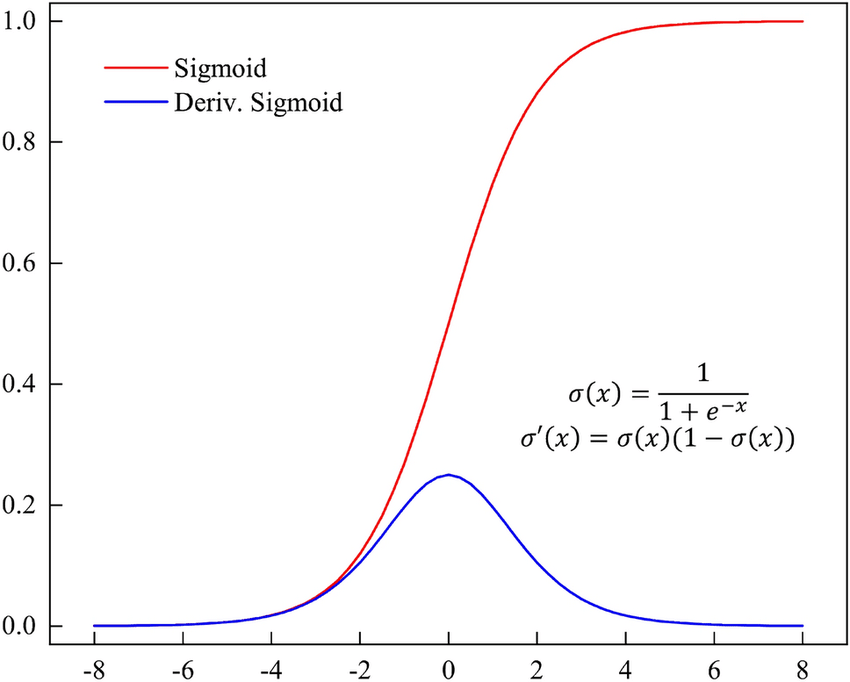
\includegraphics[width=1.00\textwidth]
                    {./images/activation_functions/xiang22_sigmoid_and_derivative.png}\\
                {\tiny 
                    \color{col:attribution} 
                    Schematic taken from Fig. 6 in \cite{Xiang:2022ato}.\\
                }
            \end{center}        
        \end{column}
        \begin{column}{0.50\textwidth}
            The \index{sigmoid}\gls{sigmoid} 
            \index{activation function}\gls{activation function},
            has a \gls{derivative} that is
            is always $<$ 1.\\
            \begin{itemize}
                \small
                \item It is only 0.25 at its maximum.\\
            \end{itemize}
            \vspace{0.2cm}
            After $N$ layers, the gradient contains
            a factor $<0.25^N$.        
            \begin{itemize}
                \small
                \item With 20 layers, $0.25^{20} \approx 10^{-12}$.
            \end{itemize}
            \vspace{0.2cm}
            Therefore, using 
            \index{back propagation}\gls{back propagation},
            the early network layers receive vanishingly small
            weight updates.
        \end{column}
    \end{columns}

    \framebreak

    %
    %

    Possible solutions to the 
    \index{vanishing gradient}\gls{vanishing gradient} 
    problem include:

    \begin{itemize}
        \item {\bf Using a different activation function} 
        \begin{itemize}
            \small
            \item 
            For example, the \index{ReLU}\gls{relu} (see figure below)
        \end{itemize}
        \item {\bf Initializing the network with large weights}
        \begin{itemize}
            \small
            \item 
            This is motivated by the fact that the product of weights also enters in the
            calculation of the \glspl{derivative} of the 
            \gls{loss function}
            (see Eq.~\ref{eq:dL_dw1_backpropagation_1}).
        \end{itemize}
    \end{itemize}

    \begin{center}
        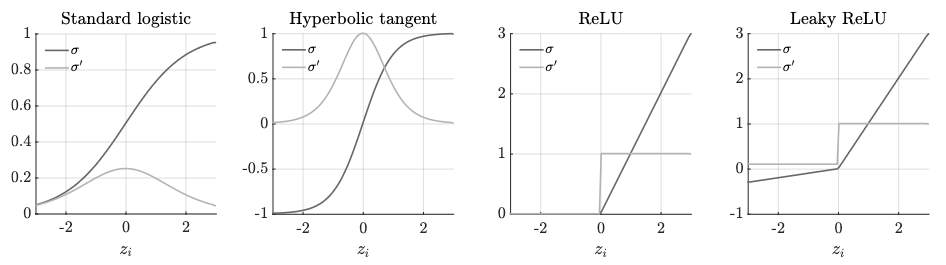
\includegraphics[width=0.99\textwidth]
            {./images/activation_functions/ostwald21_common_activation_functions_and_derivatives.png}\\
        {\tiny 
            Common activation functions and their derivatives.
            \color{col:attribution} 
            Taken from Fig. 1 in \cite{Ostwald:2021bpi}.\\
        }
    \end{center}        

    \framebreak

    %
    %

    However, these ``solutions'' to the
    \index{vanishing gradient}\gls{vanishing gradient} problem
    can cause the \gls{gradient} 
    to increase exponentially 
    along the depth of the network.
    \begin{itemize}
    \item This exponential increase is known as the 
     \index{exploding gradient}\gls{exploding gradient} problem.\\
    \end{itemize}

    Different strategies are then used to mitigate the 
    \gls{exploding gradient} problem:
    \begin{itemize}
        \item 
         \gls{gradient} clipping.\\
    \end{itemize}    
    \vspace{0.3cm}

    The
    \index{vanishing gradient}\gls{vanishing gradient} and
    \index{exploding gradient}\gls{exploding gradient} problems are
    {\bf inherent to multivariable optimization}$^1$.\\

    \vspace{0.4cm}

    \noindent\rule{4cm}{0.4pt}\\
    {
    \scriptsize
    $^1$ Although the previous observations were made for a simple network
    with a single node per layer, they are also valid for more complex networks.\\
    \begin{itemize}
        \scriptsize
        \item In the more general case, a layer-to-layer 
        \index{back propagation}\gls{back propagation} update includes 
        a (\index{Jacobian}\gls{Jacobian}) matrix (rather than scalar) multiplication         
        \cite{Aggarwal:2018SpringerDL}.
        \item Repeated matrix multiplications as unstable as
        repeated scalar ones.
    \end{itemize}
    }

    \framebreak

    %
    %

    Consider the following examples of two simple, bivariate 
    \index{loss function}\glspl{loss function}, $L$:\\
    \vspace{-0.2cm}
    \begin{equation}
        L(x,y) = 
        \begin{cases}
            x^2 + y^2,  & \text{example A} \\
            x^2 + 4y^2, & \text{example B}
        \end{cases}
    \end{equation}

    \vspace{-0.3cm}

    In example A:\\
    \begin{itemize}
        \small
        \item The \gls{loss function} looks like a {\bf circular} bowl
        (a {\em special} case) and treats the variables $x$ and $y$ symmetrically.
        \item The negative \gls{gradient} of $L$ at any point in the 
        $(x,y)$ space points directly to the minimum of $L$.\\
    \end{itemize}

    In example B:\\
    \begin{itemize}
        \small
        \item The \gls{loss function} looks like an {\bf elliptical} bowl
        and, for a unit change in the input variables,
        $y$ contributes significantly more to the loss.
        \begin{itemize}
            \small
            \item We say that $L$ is {\em more sensitive} to $y$.
        \end{itemize}    
        \item The negative \gls{gradient} of $L$ at $(x,y)$ is only
        an {\bf instantaneous direction} of best movement and does not point
        towards the minimum of $L$.
        \begin{itemize}
            \small
            \item The \gls{gradient} is {\em weighted 
            more heavily} in the $y$ direction.
        \end{itemize}    
    \end{itemize}

    \framebreak

    %
    %

    With very few exceptions, the {\bf instantaneous direction} 
    of best movement is {\bf not the correct direction of 
    descent in the longer term}.\\

    \vspace{0.2cm}

    \begin{center}
        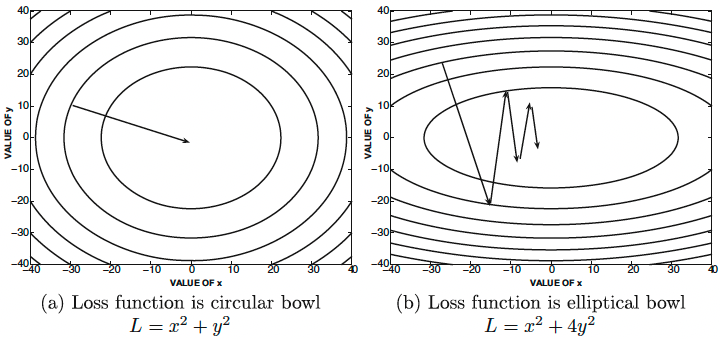
\includegraphics[width=0.80\textwidth]
            {./images/training_issues/aggarwal18_shape_loss_function_grad_descent.png}\\
        {\tiny 
           \color{col:attribution} 
            Fig. 3.9 in \cite{Aggarwal:2018SpringerDL}.\\
        }
    \end{center}        
    
    {\scriptsize
    Note that, on the right, \index{gradient descent}\gls{gradient descent}
    steps in the y direction are large, but their effect is undone in subsequent steps.
    Progress in the x direction is consistent but small.\\
    }

    \framebreak

    %
    %
    At the training \index{epoch}\gls{epoch} $k$, 
    \index{gradient descent} \gls{gradient descent}
    produces the following update:
    \begin{equation}
        \vect{w}_{k} \rightarrow 
          \vect{w}_{k+1} =  
          \vect{w}_{k} - \alpha_{k} \nabla_{w}{L(\vect{w})}
            \Big\rvert_{\vect{w} = \vect{w}_{k}}
        \label{eq:zz_grad_descent_update_k_long}    
    \end{equation}
    
    Let $\vect{g}_k$ be the 
    direction of search for the minimum of $L(\vect{w})$: 
    \begin{equation}
       \vect{g}_k = - \nabla_{w}{L(\vect{w})}
            \Big\rvert_{\vect{w} = \vect{w}_{k}}
        \label{eq:zz_line_search_direction}    
    \end{equation}
    
    Using the above definition of $\vect{g}_k$, 
    Eq.~\ref{eq:zz_grad_descent_update_k_long} can be written compactly as:
    \begin{equation}
        \vect{w}_{k} \rightarrow 
          \vect{w}_{k+1} =  
          \vect{w}_{k} + \alpha_{k} \vect{g}_{k}
        \label{eq:zz_grad_descent_update_k}    
    \end{equation}
    
    The \gls{gradient descent} update in 
    Eq.~\ref{eq:zz_grad_descent_update_k} minimises
    $L(\vect{w}_{k+1})$:
    \begin{equation}
        \frac{\partial L(\vect{w}_{k+1})}{\partial \alpha_{k}} = 0
        \label{eq:zz_condition_to_minimize_L}    
    \end{equation}
    
    Using Eqs.~\ref{eq:zz_line_search_direction} 
    and \ref{eq:zz_grad_descent_update_k}, 
    the left-hand side of Eq.~\ref{eq:zz_condition_to_minimize_L}
    yields:
    \begin{equation}
          \frac{\partial L(\vect{w}_{k+1})}{\partial \alpha_{k}} =
           \Bigg(\nabla_{\vect{w}} L(\vect{w})
             \Big\rvert_{\vect{w} = \vect{w}_{k+1}} \Bigg)^T \cdot
           \frac{\partial \vect{w}_{k+1}}{\partial \alpha_{k}} =
           - \vect{g}_{k+1}^T \cdot \vect{g}_{k}
        \label{eq:zz_grad_L_wrt_a_k}    
    \end{equation}
    
    From Eqs.~\ref{eq:zz_condition_to_minimize_L}
    and \ref{eq:zz_grad_L_wrt_a_k}, we see that:
    \begin{equation}
        \vect{g}_{k+1}^T \cdot \vect{g}_{k} = 0
        \label{eq:zz_orthogonal_updates_1}    
    \end{equation}
    
    Therefore, {\bf the directions of search at the training 
    \index{epoch}\glspl{epoch} 
    $k$ and $k+1$ are guaranteed to be orthogonal}!\\
    \vspace{0.2cm}
    
    Indeed, as a result of Eq.~\ref{eq:zz_orthogonal_updates_1},
    we find that:
    \begin{equation}
      \Big(\vect{w}_{k+2}-\vect{w}_{k+1}\Big)^T \cdot
      \Big(\vect{w}_{k+1}-\vect{w}_{k}\Big) = 
      % \Big(\alpha_{k+1} \vect{g}_{k+1}\Big)^T \cdot
      % \Big(\alpha_{k} \vect{g}_{k}\Big) = 
      \alpha_{k+1} \alpha_{k} \vect{g}_{k+1}^T \cdot \vect{g}_{k} = 0
      \label{eq:zz_orthogonal_updates_2}    
    \end{equation}
        
    \framebreak

    %
    %

    If the instantaneous direction of best movement 
    not the correct direction of 
    descent in the longer term, then one needs to:
    \begin{itemize}
        \item take only a small step, and
        \item calculate a course correction.
    \end{itemize}    

    \vspace{0.1cm}

    In this case, our \index{optimisation}\gls{optimisation} procedure 
    is forced to make a {\bf large number of iterations},
    which can become very {\bf inefficient}.\\

    \vspace{0.2cm}

    The \index{vanishing gradient}\glspl{vanishing gradient} 
    is an {\bf extreme manifestation}
    of a behaviour that characterises most
    \index{optimisation}\gls{optimisation} tasks using
    \index{gradient descent}\gls{gradient descent}.\\

\end{frame}

%  - Leaky ReLU and maxout 
\subsection{Local minima}


\begin{frame}[t,allowframebreaks]{
    Local minima -}

    A convex \index{optimisation}\gls{optimisation} 
    problem is reduced to finding a 
    \index{local minimum}\gls{local minimum}.
    \begin{itemize}
        \item A \gls{local minimum} is guaranteed to be a
        \index{global minimum}\gls{global minimum}.\\
    \end{itemize}

    \vspace{0.1cm}

    \index{neural network}\Glspl{neural network} with non-linear 
    \index{activation function}\glspl{activation function}
    yield a nonconvex \index{loss function}\gls{loss function}.\\
    \vspace{0.1cm}

    A nonconvex function, 
    can have multiple \glspl{local minimum}.

    \begin{columns}[t]
        \begin{column}{0.40\textwidth}
            \begin{center}
                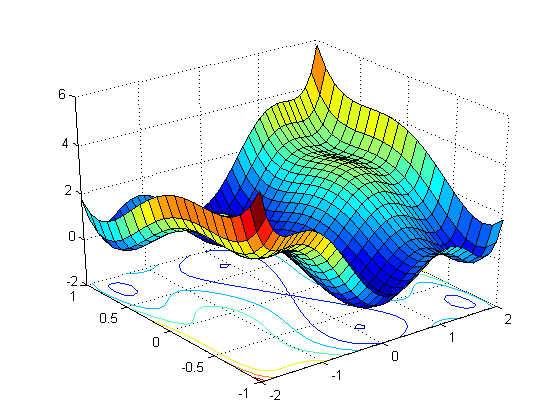
\includegraphics[width=0.98\textwidth]
                    {./images/training_issues/local_minima_illustration.png}\\
                {\tiny 
                    \color{col:attribution} 
                    Taken from \cite{StackExch:MultipleMinima}.\\    
                }
            \end{center}                        
        \end{column}
        \begin{column}{0.60\textwidth}
        \end{column}
    \end{columns}

\end{frame}

\section{Gradient descent strategies}

\subsection{Learning rate decay}

\begin{frame}[t,allowframebreaks]{
    Learning rate decay -}

\end{frame}


\subsection{Momentum-based strategies}

\begin{frame}[t,allowframebreaks]{
    Momentum-based learning -}

    As the instantaneous direction of best movement is very rarely 
    the correct direction of descent, 
    \index{optimisation}\gls{optimisation} 
    often follows a zigzag trajectory.\\
    \vspace{0.2cm}
    \index{momentum}\Gls{momentum}-based methods \cite{Polyak:1964a}
    improve the  
    \index{gradient descent}\gls{gradient descent}, 
    by following an 
    {\bf {\em `averaged'} direction towards the minimum} 
    of the \index{loss function}\gls{loss function}.\\
    \begin{columns}
        \begin{column}{0.50\textwidth}
            \begin{center}
                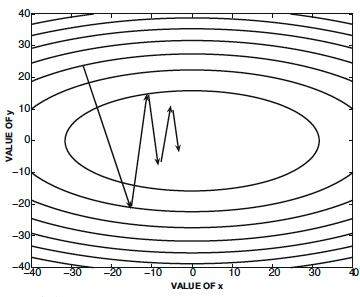
\includegraphics[width=0.98\textwidth]
                    {./images/training_issues/aggarwal18_shape_loss_function_grad_descent_R.png}\\
                {\tiny 
                    \color{col:attribution} 
                    Taken from Fig. 3.9 in \cite{Aggarwal:2018SpringerDL}.\\    
                }
            \end{center}                
        \end{column}
        \begin{column}{0.50\textwidth}
            \begin{itemize}
                \item
                The algorithm allows {\bf inertia}$^{1}$ 
                in the direction of descent.\\
                \begin{itemize}
                    \small
                    \item Builds inertia adding 
                    a new term to the parameter update rule.
                \end{itemize}
                \item
                The inertia helps to alleviate the amplitude 
                of oscillations from noisy 
                \index{gradient}\glspl{gradient}.\\
                \item
                By avoiding zigzagging, learning is accelerated.\\
            \end{itemize}
        \end{column}
    \end{columns}

    \framebreak

    %
    %
 
    In the plain \index{gradient descent}\gls{gradient descent}
    method, the parameter update is given by:
    \begin{equation}
        \vect{w}_{k} \rightarrow \vect{w}_{k+1} = 
            \vect{w}_{k} + \delta \vect{w}_{k} 
    \end{equation}\\
    where 
    \begin{equation}
        \delta \vect{w}_{k} = - \alpha \nabla_{\vect{w}} L(\vect{w}_{k})
    \end{equation}\\

    In the \index{momentum}\gls{momentum}-based method,
    the update rule is modified so that: 
    \begin{equation}
        \delta \vect{w}_{k} = 
          - \alpha \nabla_{\vect{w}} L(\vect{w}_{k})
          + \beta \delta \vect{w}_{k-1}
        \label{eq:momentum_method_update_rule}
    \end{equation}
    where $\beta$ $\in (0,1)$ is the 
    \index{momentum parameter}\gls{momentum parameter}.\\

    \vspace{0.2cm}

    Often, the step size, $\delta \vect{w}_{k}$, is referred to as the 
    \index{velocity}\gls{velocity},
    and the parameter $\beta$ as the 
    \index{friction parameter}\gls{friction parameter}.\\

    \framebreak

    %
    %

    As we've seen, in the \index{momentum}\gls{momentum}-based method,
    the update rule becomes: 
    \begin{equation*}
        \delta \vect{w}_{k} = 
          - \alpha \nabla_{\vect{w}} L(\vect{w}_{k})
          + \beta \delta \vect{w}_{k-1}
    \end{equation*}
    
    \begin{columns}[t]
        \begin{column}{0.60\textwidth}
            Larger values of 
            $\beta$, help to pick up a 
            \index{velocity}\gls{velocity} 
            towards the correct direction.\\
            \begin{center}
                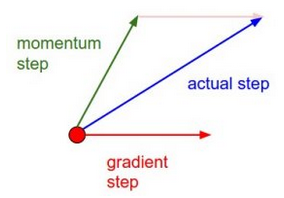
\includegraphics[width=0.50\textwidth]
                    {./images/training_issues/cs231n_momentum_update.png}\\
                {\tiny 
                    \color{col:attribution} 
                    Taken from \cite{CS231n}.\\    
                }
            \end{center}                
            The \gls{velocity} allows an effective 
            dumping of large sideways perturbations.\\        
        \end{column}
        \begin{column}{0.40\textwidth}
            \vspace{-0.5cm}
            \begin{center}
                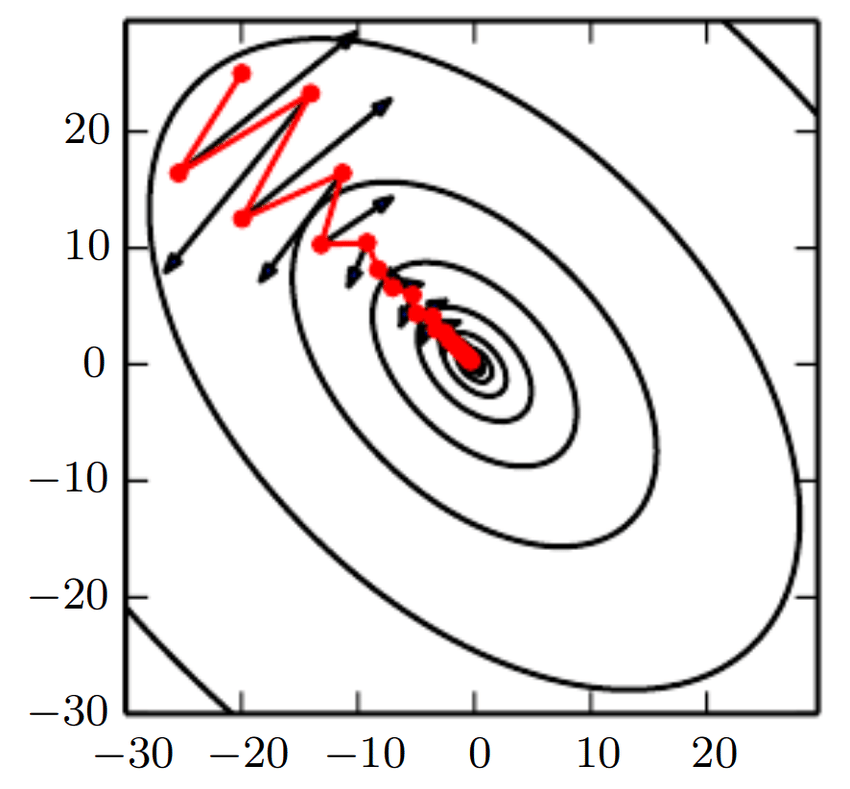
\includegraphics[width=0.98\textwidth]
                    {./images/training_issues/goodfellow17_search_path_w_momentum.png}\\
                {\scriptsize
                  Black: \index{gradient}\gls{gradient} step.
                  Red: actual step of \gls{momentum}-based method.\\
                }
                {\tiny 
                    \color{col:attribution} 
                    Taken from Fig. 8.5 in \cite{Goodfellow:2017MITDL}.\\    
                }
            \end{center}                
        \end{column}
    \end{columns}

    \framebreak

    %
    %

    The \index{momentum}\gls{momentum}-based methods {\bf overshoot} in 
    the direction of \index{velocity}\gls{velocity}.
    \begin{itemize}
        \small
        \item Similarly as a ball rolling down a bowl will overshoot the minimum.
    \end{itemize}    
    \vspace{0.1cm}
    Nevertheless, \gls{momentum}-based methods perform better.
    \begin{itemize}
        \small
        \item Faster approach to the minimum
        more than compensates for overshooting.
    \end{itemize}    
    \vspace{0.1cm}
    Overshooting can be beneficial to the extend it helps escape local minima.\\

    \begin{center}
        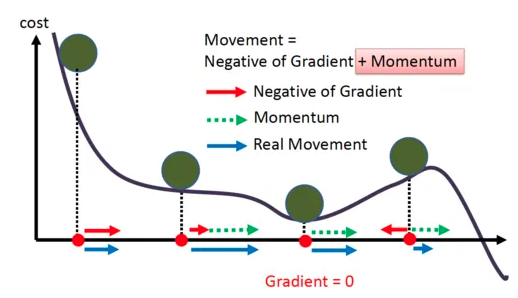
\includegraphics[width=0.60\textwidth]
            {./images/training_issues/khandewal20_gradient_descent_ball.png}\\
        {\tiny 
            \color{col:attribution} 
            Taken from \cite{Medium:GradDescentMomRMSPropAdam}.\\    
        }
    \end{center}                        

    \framebreak

    %
    %

    To elucidate the previous formulas, study the following pseudo-code.\\
    \vspace{0.1cm}
    \begin{block}{
        Mini-batch \index{gradient descent}\gls{gradient descent}
        with \index{momentum}\gls{momentum}}
    {\tt \scriptsize
       {\bf Set} hyperparameters 
       (learning rate $\alpha$, momentum parameter $\beta$) to desired values\\
       \vspace{0.1cm}
       {\bf Randomize} initial set of network weights, $\vect{w}_{0}$\\
       \vspace{0.1cm}
       {\bf Initialize} auxiliary variables: $k=-1$, $\delta \vect{w}_{-1} = 0$\\
       \vspace{0.1cm}
       {\bf While} [convergence condition not met]:\\
       \vspace{0.1cm}
       \begin{itemize}        
        {\scriptsize
        \item Increment $k$
        \vspace{0.2cm}
        \item Sample a minibatch of $N$ training examples 
        $(\vect{x}_i, y_i)$
        \item Compute the loss gradient:
        $\displaystyle g_k = \frac{1}{N} \nabla_{\vect{w}} 
          \sum_{i=0}^{N-1} L\Big(f(\vect{x}_i, \vect{w}_{k}),y_i\Big)$ 
        \item Compute the velocity update: $\delta \vect{w}_{k} =  
                - \alpha g_k
                + \beta \delta \vect{w}_{k-1}$\\
        \vspace{0.2cm}
        \item Apply the update to the network parameters: 
              $\vect{w}_{k+1} = \vect{w}_{k} + \delta \vect{w}_{k}$
        }
       \end{itemize}
       {\bf End while}
    }
    \end{block}

    \framebreak

    %
    %

    Following the first few steps of the algorithm, 
    we find for the {\em velocity}:

    \begin{equation*}
        \delta \vect{w}_{0} = 
        - \alpha \nabla_{\vect{w}} L(\vect{w}_{0})
        + \beta \cancelto{0}{\delta \vect{w}_{-1}}
    \end{equation*}

    \vspace{-0.1cm}

    \begin{equation*}
        \delta \vect{w}_{1} = 
        - \alpha \nabla_{\vect{w}} L(\vect{w}_{1})
        + \beta \delta \vect{w}_{0} =
        - \alpha \Big(
            \nabla_{\vect{w}} L(\vect{w}_{1}) +
            \beta \nabla_{\vect{w}} L(\vect{w}_{0})
        \Big)
    \end{equation*}

    \vspace{-0.4cm}

    \begin{equation*}
        \delta \vect{w}_{2} = 
        - \alpha \nabla_{\vect{w}} L(\vect{w}_{2})
        + \beta \delta \vect{w}_{1} = %\Rightarrow
        - \alpha \Big(
            \nabla_{\vect{w}} L(\vect{w}_{2}) +
            \beta \nabla_{\vect{w}} L(\vect{w}_{1}) +
            \beta^2 \nabla_{\vect{w}} L(\vect{w}_{0})
        \Big)
    \end{equation*}

    \begin{equation*}
        \cdots
    \end{equation*}

    \vspace{0.1cm}

    This generalizes to:\\

    \vspace{-0.4cm}

    \begin{equation}
        \frac{-\delta \vect{w}_{k}}{\alpha} = 
            \nabla_{\vect{w}} L(\vect{w}_{k}) +
            \beta \nabla_{\vect{w}} L(\vect{w}_{k-1}) +
            \beta^2 \nabla_{\vect{w}} L(\vect{w}_{k-2}) + 
            \cdots + 
            \beta^k \nabla_{\vect{w}} L(\vect{w}_{0}) 
        \label{eq:grad_descent_momentum_step_k}
    \end{equation}

    \framebreak

    %
    %

    As we observe from Eq.~\ref{eq:grad_descent_momentum_step_k}
    \begin{equation*}
        \frac{-\delta \vect{w}_{k}}{\alpha} = 
            \nabla_{\vect{w}} L(\vect{w}_{k}) +
            \beta \nabla_{\vect{w}} L(\vect{w}_{k-1}) +
            \beta^2 \nabla_{\vect{w}} L(\vect{w}_{k-2}) + 
            \cdots + 
            \beta^k \nabla_{\vect{w}} L(\vect{w}_{0}) 
    \end{equation*}

    the \index{velocity}\gls{velocity} 
    $\delta \vect{w}_{k}$ {\bf accumulates \index{gradient}\glspl{gradient}}.

    \vspace{0.2cm}

    \Glspl{gradient} from further back in the past of the 
    \index{optimisation}\gls{optimisation} process, 
    are weighted with a higher power of 
    the \index{momentum parameter}\gls{momentum parameter} $\beta$ ($\in (0,1)$).

    \vspace{0.2cm}

    The \gls{velocity} $\delta \vect{w}_{k}$ is an 
    {\bf exponentially decaying moving average of past gradients}.

    \framebreak

    %
    %

    We note that the step depends on the size 
    and {\bf alignment} of the gradients.\\
    \vspace{0.2cm}

    If the code observed a constant gradient $\vect{g}$, 
    Eq. \ref{eq:grad_descent_momentum_step_k} becomes:\\
    \begin{equation}
        \delta \vect{w}_{k} = 
            -\alpha \vect{g} \Big(
               1 + \beta + \beta^2 + \cdots + \beta^k
            \Big)
    \end{equation}

    Above, we recognise a geometric series 
    written in closed form as:\\
    \begin{equation}
        1 + \beta + \beta^2 + \cdots + \beta^k = \frac{1}{1-\beta}
    \end{equation}

    Therefore, the velocity reaches a {\em terminal} value of:\\
    \begin{equation}
        \delta \vect{w}_{k} = 
            \frac{-\alpha \vect{g}}{1-\beta} \Rightarrow
        |\delta \vect{w}_{k}| = 
            \frac{\alpha |\vect{g}|}{1-\beta} 
    \end{equation}

    \vspace{0.1cm}

    For $\beta$=0.9, 
    the typical gradient descent step, $\alpha |\vect{g}|$,
    for this situation,
    is increased by a factor $1/(1-\beta)$=10.\\
    % \vspace{0.1cm}
    % \noindent\rule{4cm}{0.4pt}\\
    % {\scriptsize
    % $^{(1)}$ For $|r|<$1, $\displaystyle \sum_{k=0}^{\infty}ar^k = \frac{a}{1-r}$.
    % }

\end{frame}


\subsubsection{Nesterov momentum}




\begin{frame}[t,allowframebreaks]{
    Momentum-based learning: Nesterov momentum -}

    \index{Nesterov momentum}\gls{Nesterov momentum} \cite{Nesterov:1983a}
    is a {\bf variant of the \index{momentum}\gls{momentum}}-based method.\\
    \vspace{0.2cm}
    In this algorithm, the update rule is given by:\\
    \vspace{-0.2cm}
    \begin{equation}
        \delta \vect{w}_{k} = 
          - \alpha \nabla_{\vect{w}} L(\vect{w}_{k}+\beta \delta \vect{w}_{k-1})
          + \beta \delta \vect{w}_{k-1}
        \label{eq:momentum_method_update_rule}
    \end{equation}
    \vspace{0.1cm}
    The only difference is that the \index{gradient}\gls{gradient}
    of the \index{loss function}\gls{loss function}, at step $k$, 
    is evaluated at $\vect{w}=\vect{w}_{k}+\beta \delta \vect{w}_{k-1}$
    rather than at $\vect{w}=\vect{w}_{k}$,
    \begin{itemize}
        \item i.e., the \gls{gradient} is 
        {\bf evaluated after adding the current \index{velocity}\gls{velocity}}.\\
    \end{itemize}

    \begin{center}
        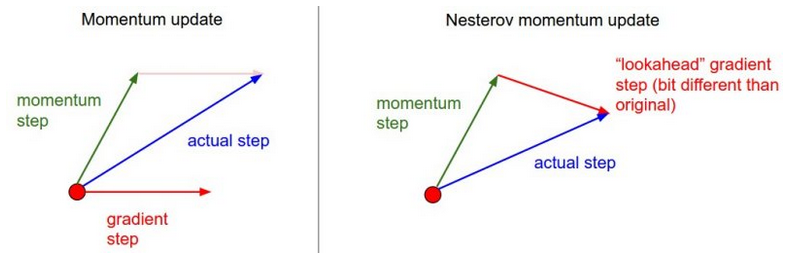
\includegraphics[width=0.80\textwidth]
            {./images/training_issues/cs231n_momentum_update_nesterov.png}\\
        {\tiny 
            \color{col:attribution} 
            Taken from \cite{CS231n}.\\    
        }
    \end{center}                

    \framebreak

    %
    %

    By {\bf looking ahead}
    (and evaluating the gradient after adding the \index{velocity}\gls{velocity}),
    \index{momentum}\index{Nesterov momentum}\gls{Nesterov momentum} 
    makes a correction to {\bf avoid overshooting}.\\

    \begin{center}
        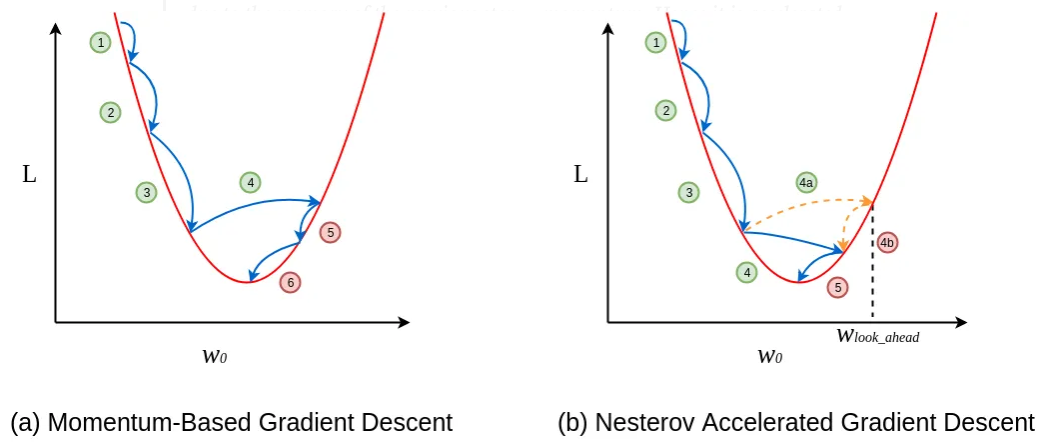
\includegraphics[width=0.88\textwidth]
            {./images/training_issues/chandra19_nesterov_momentum_updates.png}\\
        \vspace{0.1cm}
        {\scriptsize
            The plain \gls{momentum} method, based on reinforcement from previous 
            updates, takes a large step in update 4 and overshoots the minimum.
            It then recovers in steps 5 and 6.\\
            \gls{Nesterov momentum}, looks ahead before taking step 4, 
            and exploits that changing sign of the \index{gradient}\gls{gradient} 
             to try a smaller step.
            \color{col:attribution} 
            Taken from \cite{TowardsDataScience:LP2MomentumBasedGS}.\\    
        }
    \end{center}   
    
\end{frame}


\subsection{Adaptive sub-gradient methods}


\begin{frame}[t,allowframebreaks]{
    Adaptive subgradient algorithms -}

    The \index{learning rate}\gls{learning rate}
    is {\em `the single most important 
    \index{hyperparameter}\gls{hyperparameter}'} \cite{Bengio:2012gbt},
    but it is also {\bf one of the most difficult ones to adjust}.\\
    \begin{itemize}
        \small
        \item
        A key issue is this that
        the \index{loss function}\gls{loss function} has 
        {\bf greatly-varying levels of sensitivity} to changes 
        in different directions in its parameter space.\\
    \end{itemize}

    \vspace{0.2cm}

    The \index{momentum}\gls{momentum}-based methods
    alleviates the problem, 
    but at the expense of adding another \gls{hyperparameter}
    (the \index{momentum parameter}\gls{momentum parameter}).

    \vspace{0.2cm}

    An obvious alternative approach is to {\bf choose a different 
    \gls{learning rate} for each direction} in the parameter space.\\
    \begin{itemize}
        \small
        \item This is challenging, since networks 
        can have {\bf millions or parameters}.
    \end{itemize}

    \vspace{0.2cm}

    There exist several such 
    \index{adaptive subgradient}\gls{adaptive subgradient} algorithms.\\
    \begin{itemize}
        \small
        \item 
        We will study a few well-known variants of this 
        class of algorithms, such as 
        \index{delta-bar-delta}\gls{delta-bar-delta} \cite{Jacobs:1988dbd},
        \index{AdaGrad}\gls{AdaGrad} \cite{Duchi:11a},
        \index{RMSProp}\gls{RMSProp} \cite{Hinton:2012rmsp}, and
        \index{Adam}\gls{Adam} \cite{Kingma:2017adam}.
    \end{itemize}

    \framebreak
 
    %
    %
    \index{adaptive subgradient}\Gls{adaptive subgradient} algorithms
    extends the learning rule used in 
    the plain gradient descent method
    \begin{equation}
        \vect{w}_{k} \rightarrow \vect{w}_{k+1} = 
        \vect{w}_{k} + \delta \vect{w}_{k} =
        \vect{w}_{k} - \alpha \nabla_{\vect{w}} L(\vect{w}_{k})
    \end{equation}\\
    to
    \begin{equation}
        \vect{w}_{k} \rightarrow \vect{w}_{k+1} = 
        \vect{w}_{k} + \delta \vect{w}_{k} =
        \vect{w}_{k} - \vect{\alpha}_{k} \odot \nabla_{\vect{w}} L(\vect{w}_{k})
        \label{eq:subgradient_method_learning_rule}
    \end{equation}\\
    where
    the constant scalar \index{learning rate}\gls{learning rate} $\alpha$ 
    is expanded to a vector $\vect{\alpha}_{k}$ 
    with values that depend on the epoch $k$$^1$.\\

    \vspace{0.2cm}

    Each element of the vector $\vect{\alpha}_{k}$ is the 
    {\bf individual and constantly updated \gls{learning rate} 
    corresponding to a distinct weight}.\\
     
    \vspace{0.2cm}
    \noindent\rule{4cm}{0.4pt}\\
    {\small
        $^1$ In Eq.~\ref{eq:subgradient_method_learning_rule}, $\odot$ denotes
        an element-wise multiplication of the two vectors.\\
    }

\end{frame}


\subsubsection{Delta-bar-delta algorithm}


\begin{frame}[t,allowframebreaks]{
    Adaptive subgradient algorithms: delta-bar-delta -}

    \index{delta-bar-delta}\Gls{delta-bar-delta} \cite{Jacobs:1988dbd}
    is an early, {\bf heuristic}
    \index{adaptive subgradient}\gls{adaptive subgradient} algorithm.\\

    

\end{frame}
\subsubsection{AdaGrad algorithm}



\begin{frame}[t,allowframebreaks]{
    Adaptive subgradient algorithms: AdaGrad -}

    \index{AdaGrad}\gls{AdaGrad} \cite{Duchi:11a} adapts the 
    \index{learning rate}\glspl{learning rate} 
    for each individual model parameter.\\
    \vspace{0.2cm}

    The \glspl{learning rate} are scaled inversely proportional to 
    the square root of the running sum of 
    the squared \index{gradient}\gls{gradient} 
    of the \index{loss function}\gls{loss function}.

    \begin{equation}
          \displaystyle
          \alpha_k \leftarrow 
          \frac{\alpha}
          {\sqrt{\sum_{\ell=0}^{k-1} 
            \Big(\frac{\partial L}{\partial w}\Big)^2}}
        \label{eq:adagrad_rate_update_rule}
    \end{equation}

\end{frame}
\subsubsection{RMSprop algorithm}



\begin{frame}[t,allowframebreaks]{
    Adaptive subgradient algorithms: RMSProp -}

\end{frame}
\subsubsection{Adam algorithm}


\begin{frame}[t,allowframebreaks]{
    Adaptive subgradient algorithms: Adam -}

\end{frame}
\subsection{Second-order methods}

\begin{frame}[t,allowframebreaks]{
    Beyond the gradient: Second-order methods -}

    The methods outlined previously, improve upon the plain
    \index{gradient descent}\gls{gradient descent} method,
    using only the \index{gradient}\gls{gradient}.\\
    \vspace{0.2cm}
    \index{second-order method}\Glspl{second-order method}
    is a class of \index{optimisation}\gls{optimisation} methods
    {\bf making use of the second derivatives of the 
    \index{loss function}\gls{loss function}}.\\
    \vspace{0.2cm}
    A simple and widely-used \gls{second-order method} is
    \index{Newton's method}{\bf \gls{Newton's method}}.\\
    \begin{itemize}
        \small
        \item \gls{Newton's method} is {\bf inefficient} except 
        for networks with few parameters.\\ 
        \item At each training \index{epoch}\gls{epoch}, 
        it requires the inversion of a
        \index{Hessian}\gls{Hessian} matrix with
        dimensions $N \times N$, where $N$ is the 
        number of parameters. 
    \end{itemize}
    \vspace{0.2cm}
    There exist several {\bf approximate \glspl{second-order method}} 
    avoiding computing the inverse \gls{Hessian} matrix:
    \begin{itemize}
        \item \index{conjugate gradients}\Gls{conjugate gradients}
        \item \index{BFGS}\gls{bfgs} 
        \item \index{L-BFGS}\gls{lbfgs} 
    \end{itemize}

\end{frame}

\subsubsection{Newton's method}


\begin{frame}[t,allowframebreaks]{
    Second-order methods: Netwon's method -}

    \index{Newton's method}\gls{Newton's method} uses a second-order
    \index{Taylor series}\gls{Taylor series} 
    (see Eq.~\ref{eq:hessian_taylor_1})
    of the \index{loss function}\gls{loss function}, $L(\vect{w})$
    around a point $\vect{w}_0$:\\
    \vspace{-0.2cm}
    \begin{equation}
        L(\vect{w}) \approx 
          L_0 + 
          (\vect{w}- \vect{w}_0)^T \cdot \vect{g} +
          \frac{1}{2} (\vect{w} - \vect{w}_0)^T \cdot 
            \vect{H} \cdot (\vect{w} - \vect{w}_0)
        \label{eq:newton_quadratic_loss_approximation}    
    \end{equation}

    where $L_0$ is the \gls{loss function}, $L(\vect{w})$,
    evaluated at $\vect{w}_0$:\\
    \vspace{-0.2cm}
    \begin{equation}
        L_0 = L(\vect{w}) \Big\rvert_{\vect{w}=\vect{w}_0},
    \end{equation}
    
    $\vect{g}$ is the \index{gradient}\gls{gradient} 
    of $L(\vect{w})$ evaluated at $\vect{w}_0$:\\
    \vspace{-0.2cm}
    \begin{equation}
        \vect{g} = \nabla_{\vect{w}}L(\vect{w}) \Big\rvert_{\vect{w}=\vect{w}_0},
    \end{equation}\\

    and $\vect{H}$ is the \index{Hessian matrix}\gls{Hessian matrix} 
    (see Eq.~\ref{eq:hessian_1}) of $L(\vect{w})$, 
    with elements $H_{ij}$ that are also evaluated at $\vect{w}_0$:\\
    \vspace{-0.2cm}
    \begin{equation}
        H_{ij} = 
        \frac{\partial^2 L(\vect{w})}{\partial w_i \partial w_j}
        \Big\rvert_{\vect{w}=\vect{w}_0}.
    \end{equation}\\

    \framebreak
 
    %
    %

    Finding the \index{critical point}\gls{critical point}, 
    of the function $L(\vect{w})$ requires solving:
    \begin{equation}
        \nabla_{\vect{w}} L(\vect{w}) = 0. 
        \label{eq:newton_citical_point_condition_1}    
    \end{equation}
    Substituting Eq.~\ref{eq:newton_quadratic_loss_approximation}
    in Eq.~\ref{eq:newton_citical_point_condition_1}, we can write:
    \begin{equation}
        \nabla_{\vect{w}} \Big( 
            L_0 + 
            \sum_{i} (w_{i} - w_{i0}) g_{i} +
            \frac{1}{2} \sum_{i,j} (w_{i} - w_{i0}) H_{ij} (w_j - w_{j0})
        \Big) = 0 
        \label{eq:newton_citical_point_condition_2}    
    \end{equation}
    In the above expression, all vector and matrix multiplications
    are shown explicitly for clarity.\\
    \vspace{0.2cm}
    Calculating the \index{gradient}\gls{gradient} 
    in Eq.~\ref{eq:newton_citical_point_condition_2} yields:
    \begin{equation}
        \vect{g} + \vect{H} (\vect{w} - \vect{w}_{0}) = 0.
        \label{eq:newton_gradient_of_quadratic_loss}    
    \end{equation}
    \vspace{0.2cm}
    A detailed derivation is given in the following page.\\


    \framebreak
 
    %
    %

    \begin{equation*}
        \scriptsize
        \nabla_{\vect{w}} \Big( 
            L_0 + 
            \sum_{i} (w_{i} - w_{i0}) g_{i} +
            \frac{1}{2} \sum_{i,j} (w_{i} - w_{i0}) H_{ij} (w_j - w_{j0})
        \Big) = 
    \end{equation*}
    \begin{equation*}
        \scriptsize
        \sum_{k} \vect{\hat{k}} \frac{\partial}{\partial w_k}
        \Big( 
            L_0 + 
            \sum_{i} (w_{i} - w_{i0}) g_{i} +
            \frac{1}{2} \sum_{i,j} (w_{i} - w_{i0}) H_{ij} (w_j - w_{j0})
        \Big) = 
    \end{equation*}
    \begin{equation*}
        \scriptsize
        \sum_{k} \vect{\hat{k}} 
        \Bigg( 
            \cancelto{0}{\frac{\partial L_0}{\partial w_k}}
            + 
            \sum_{i} 
            \frac{\partial (w_{i} - w_{i0})}{\partial w_k}
             g_{i} +
            \frac{1}{2} 
            \sum_{i,j} 
            \Big\{
                \frac{\partial (w_{i} - w_{i0})}{\partial w_k} H_{ij} (w_j - w_{j0}) +
                (w_{i} - w_{i0}) H_{ij} \frac{\partial (w_j - w_{j0})}{\partial w_k}
            \Big\}            
        \Bigg) = 
    \end{equation*}
    \begin{equation*}
        \scriptsize
        \sum_{k} \vect{\hat{k}} 
        \Bigg( 
            \sum_{i} 
            \delta_{ki}
             g_{i} +
            \frac{1}{2} 
            \sum_{i,j} 
            \Big\{
                \delta_{ki} H_{ij} (w_j - w_{j0}) +
                (w_{i} - w_{i0}) H_{ij} \delta_{kj}
            \Big\}            
        \Bigg) = 
    \end{equation*}
    \begin{equation*}
        \scriptsize
        \sum_{k} \vect{\hat{k}} 
        \Big( 
            \sum_{i} 
                \delta_{ki}
                g_{i} +
            \cancel{\frac{1}{2}}
                \sum_{i,j}
                \cancel{2} \delta_{ki} H_{ij} (w_j - w_{j0}) 
        \Big) = 
    \end{equation*}
    \begin{equation*}
        \scriptsize
        \sum_{i} 
            \vect{\hat{i}}
            g_{i} +
        \sum_{i,j}
            \vect{\hat{i}}
            H_{ij} (w_j - w_{j0}) 
            = 0 \Rightarrow
    \end{equation*}

    \begin{equation*}
        \scriptsize
        \vect{g} + \vect{H} (\vect{w} - \vect{w}_{0}) = 0
    \end{equation*}

    \framebreak
 
    %
    %

    From Eq.~\ref{eq:newton_gradient_of_quadratic_loss},    
    we can find$^1$
    the \gls{critical point}, $\vect{w}^{\star}$,
    of the function $L(\vect{w})$:
    \begin{equation}
        \vect{w}^{\star} = \vect{w}_{0} - \vect{H}^{-1} \vect{g}
        \label{eq:newton_critical_point}    
    \end{equation}
    
    This expression suggests that, 
    we can leap directly to the minimum of $L(\vect{w})$ by 
    scaling the \index{gradient}\gls{gradient}, $\vect{g}$, 
    with the inverse of the \index{Hessian matrix}\gls{Hessian}, 
    $\vect{H}^{-1}$.\\

    \vspace{0.2cm}

    Note that we {\em assumed} a {\bf locally quadratic} function
    with a \gls{Hessian} that is 
    \index{positive definite}{\bf \gls{positive definite}}.\\

    \vspace{0.2cm}

    For a function that are is not locally quadratic, we can apply 
    \index{Newton's method}\gls{Newton's method} {\bf iteratively},
    as long as the \gls{Hessian} is \gls{positive definite}.\\

    \vspace{0.2cm}
    \noindent\rule{4cm}{0.4pt}\\
    {
        \footnotesize        
        \begin{equation*}
            ^{1}\;\;\vect{g} + \vect{H} (\vect{w}^{\star} - \vect{w}_{0}) = 0 \Rightarrow
            \vect{H}^{-1} \vect{g} + 
            \cancelto{\vect{I}}{\vect{H}^{-1}\vect{H}} (\vect{w}^{\star} - \vect{w}_{0}) = 0 \Rightarrow
            \vect{w}^{\star} = \vect{w}_{0} - \vect{H}^{-1} \vect{g}
        \end{equation*}    
    }

    \framebreak
 
    %
    %

    \index{Newton's method}\gls{Newton's method} is {\bf suitable only
    if the \index{Hessian matrix}\gls{Hessian} is 
    \index{positive definite}\gls{positive definite}}.\\
    \vspace{0.2cm}

    However, in deep learning,  
    the \index{loss function}\gls{loss function} is typically
    nonconvex.\\
    \begin{itemize}
        \small
        \item For example, near a \index{saddle point}
        the \gls{Hessian} is not \gls{positive definite}.
        \item In this case, \gls{Newton's method} can
        update weights in the wrong direction.
    \end{itemize}
    \vspace{0.2cm}
    If the \gls{Hessian} is not \gls{positive definite}
    it is often necessary to {\bf regularize} it.\\
    \vspace{0.1cm}
    A common strategy is to add a number 
    $\epsilon$ in the diagonal of the \gls{Hessian}:
    \begin{equation}
        \vect{w}^{\star} = \vect{w}_{0} - 
          \Big(\vect{H} + \epsilon \vect{I}\Big)^{-1} \vect{g}
        \label{eq:newton_critical_point_w_regularization}  
    \end{equation}
    This works well if the negative eigenvalues 
    of the \gls{Hessian} are small.\\
    \vspace{0.1cm}
    However, near points with a strong negative curvature, 
    $\epsilon$ may need to be so large that the \gls{Hessian}
    is dominated by its diagonal $\epsilon \vect{I}$!
    \begin{itemize}
        \small
        \item In this case, \gls{Newton's method} can be slower to
        converge than a first-order \index{gradient descent}\gls{gradient descent}
        algorithm with an optimised \index{learning rate}\gls{learning rate}.\\
    \end{itemize}

    \framebreak
 
    %
    %

    In addition to the challenges posed to the 
    \index{Newton's method}\gls{Newton's method} 
    by nonconvex \index{optimisation}\gls{optimisation} problems,
    examining Eq.~\ref{eq:newton_critical_point} again,
    \begin{equation*}
        \vect{w}^{\star} = \vect{w}_{0} - \vect{H}^{-1} \vect{g},
    \end{equation*}
    we notice another {\bf undesirable feature} of the method,
    from the point of view of computational efficiency.\\
    \vspace{0.2cm}

    For a network with $N$ parameters, 
    \index{Hessian matrix} $\vect{H}$ has a
    a dimension of $N \times N$.\\
    \begin{itemize}
        \small
        \item Inverting such a matrix 
        has a computational complexity of $\mathcal{O}(N^3)$.
        \item Such a matrix inversion is required at each training iteration!
    \end{itemize}
    \vspace{0.2cm}
    Clearly, this is {\bf impractical except 
    for networks with few parameters}.\\
    \vspace{0.2cm}
    As it was mentioned in the introduction to the
    \index{second-order method}\glspl{second-order method},
    a number of {\bf approximate methods} avoid that inversion. 
    \begin{itemize}
        \small
        \item 
        Commonly used methods are
        \index{conjugate gradients}\Gls{conjugate gradients},
        \index{BFGS}\gls{bfgs}, and
        \index{L-BFGS}\gls{lbfgs}.
    \end{itemize}
    
\end{frame}

\subsubsection{Approximate methods}


\begin{frame}[t,allowframebreaks]{
    Second-order methods: Approximate methods -}

\end{frame}



\subsection{Gradient clipping methods}


\section{Generalisation}

\begin{frame}[t,allowframebreaks]{Generalisation -}

    Training a \gls{ml} model {\em looks like} an optimization task.\\
    \vspace{0.1cm}
    \begin{blockexample}{}
      Typically, to train a \gls{ml} model: 
      \begin{itemize}
        \item 
        We use a \index{training set}\gls{training set} 
        that contains a number of examples, and
        \item
        define a \index{loss function}\gls{loss function},
        a measure of training error over that set.
      \end{itemize}
      The training process adjusts the model parameters
      to optimize the model performance (minimize the training error).\\
    \end{blockexample}
    \vspace{0.2cm}
    However, {\bf training a \gls{ml} model is not a pure optimization problem}.\\
    \vspace{0.2cm}
    Our \gls{ml} model should {\bf maintain a satisfactory performance 
    with new, previously unseen inputs} - 
    not just for the inputs in the training set.\\
    \vspace{0.2cm}
    Performing well for previously unseen inputs is called 
    \index{Generalisation}\gls{Generalisation}.\\
    \vspace{0.2cm}
    How to build model that generalise is one of the central problems in \gls{ml}.


    \framebreak

    %
    %

    In the linear regression example, our model
    \begin{equation}
        \hat{y} = {\mathbf x}^T \cdot {\mathbf w}
        %\label{eq:}
    \end{equation}        

    was trained using a set $\mathbb{D}$ of $N_{(train)}$
    training examples $({\mathbf x_{(train)}},y_{(train)})$, 
    by minimizing the loss function
    \begin{equation}
        L_{(train)} = \frac{1}{N_{(train)}} 
        \sum_{({\mathbf x_{(train)}},y_{(train)})  \in \mathbb{D}}
        \Big( y_{(train)} - {\mathbf x_{(train)}}^T \cdot {\mathbf w} \Big)^2
        %\label{eq:}
    \end{equation}        

    However, we also care for the test (Generalisation) error
    \begin{equation}
        L_{(test)} = \frac{1}{N_{(test)}} 
        \sum_{({\mathbf x_{(test)}},y_{(test)})  \in \mathbb{T}}
        \Big( y_{(test)} - {\mathbf x_{(test)}}^T \cdot {\mathbf w} \Big)^2
        %\label{eq:}
    \end{equation}        
    for the $N_{(test)}$ test examples $({\mathbf x_{(test)}},y_{(test)})$ 
    of the set $\mathbb{T}$.

    \framebreak

    %
    %

    What can we say about the \gls{ml} model performance on the test set,
    if we only ever see the training set?
    \begin{itemize}
        \item
        Not much, unless the test and training data sets come from the 
        {\bf same data-generating process}.    
    \end{itemize}
    \vspace{0.2cm}   
    Typically, we make assumptions known as the {\bf i.i.d. assumptions}.\\
    \vspace{0.2cm}
    The examples in the test and training sets are assumed to be:
    \begin{itemize}
        \item {\bf independent}, and
        \item {\bf identically distributed}, 
        i.e. they are drawn from the same probability distribution 
        (the data-generating distribution)
    \end{itemize}
    \vspace{0.2cm}
    With the i.i.d assumptions:
    \begin{itemize}
        \item
        we can describe the data-generating process
        with a probability distribution over a single data example, and
        \item
        study the relationship between the training and test error.
    \end{itemize}

\end{frame}


\section{Capacity, overfitting and underfitting}


\begin{frame}[t,allowframebreaks]{Underfitting and overfitting -}

    Typically, 
    we we choose model parameters that reduce the training error, 
    and then test the model performance against the test set.
    \begin{itemize}
    \item 
    Under this process, 
    the expected value of the test error 
    is greater than (or equal to)  
    the expected value of the training error.
    \end{itemize}
 
    \vspace{0.2cm}
    
    A central challenge is to:
    \begin{itemize}
     \item {\bf reduce the training error}, \underline{and}
     \item {\bf reduce the gap between the training and test error}.
    \end{itemize}
 
    \vspace{0.2cm}   
 
    Failing on either of these goals, gives rise to common model pathologies:
    \begin{itemize}
      \item \index{underfitting}\Gls{underfitting}:
      Our model does not describe the training data well,
      and {\bf we cannot obtain a sufficiently small training error}.
      \item \index{overfitting}\Gls{overfitting}:
      We obtain a small training error,
      but {\bf our model does not generalize well} and  
      the training error is large. 
    \end{itemize}
 
    \framebreak
 
    %
    %
 
    \begin{center}
         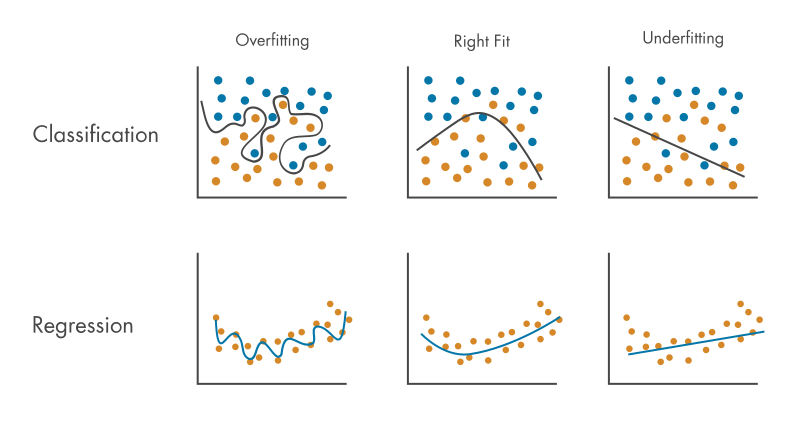
\includegraphics[width=1.0\textwidth]
             {./images/training_issues/over_and_underfitting_1.png}\\
         {\tiny 
             Illustrating overfitted and underfitted model pathologies.\\
             \color{col:attribution} 
             Schematic reproduced from \cite{MathWorks:Overfitting}.\\
         }
     \end{center}
 
 \end{frame}
 

\begin{frame}[t,allowframebreaks]{Capacity -}

    We can affect the tendency of a \gls{ml} model for 
    \index{underfitting}\gls{underfitting} or 
    \index{overfitting}\gls{overfitting},
    by adjusting its 
    \index{capacity}\gls{capacity}.\\

    \vspace{0.2cm}

    The \gls{capacity} of a model is its 
    {\bf ability to describe a broad variety of data-generating processes}.

    \vspace{0.2cm}

    \begin{itemize}
        \item 
        {\bf Models with low capacity, 
        will struggle capturing all the details} 
        of the training data and providing a satisfactory fit.\\
        % \begin{blockexample}{}
        %     \small
        %     For example, imagine using a linear model $\hat{y} = b+wx$
        %     to fit data sampled from a data-generating process with a 
        %     probability distribution that is quadratic in $x$.
        % \end{blockexample}
        \item 
        {\bf Models with high capacity 
        can memorize unimportant features} of the data
        that do not serve the purpose of model generalization.
        % \begin{blockexample}{}
        %     \small
        %     For example, imagine using a 10$^{th}$ order polynomial to
        %     to fit noisy data sampled from a data-generating process with a 
        %     probability distribution that is linear in $x$.
        % \end{blockexample}
    \end{itemize}

    \vspace{0.2cm}

    Occam's razor (the `law of parsimony')
    \cite{Wikipedia:OccamRazor} is a good guiding principle:
    Amongst competing hypotheses that describe the data equally well,
    chose the simples one.\\

    \vspace{0.2cm}

    While simpler models are likely to generalize better,
    we still need a sufficiently complex model to achieve low training error.

    \framebreak

    %
    %

    A central task in \gls{ml} is to {\bf match the capacity of the model
    to the complexity of its task and to the amount of available data.}\\

    \vspace{0.1cm}

    \begin{center}
        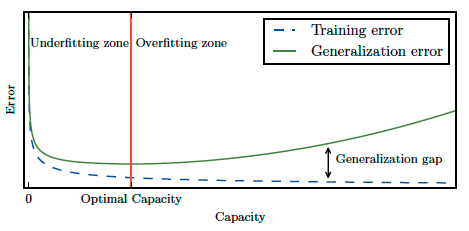
\includegraphics[width=0.90\textwidth]
            {./images/training_issues/error_vs_capacity_1.png}\\
        {\tiny 
            Illustrating the relationship between error and capacity.\\
            \color{col:attribution} 
            Schematic reproduced from p. 112 of \cite{Goodfellow:2017MITDL}.\\
        }
    \end{center}

    \framebreak

    %
    %

    There are several ways to affect the capacity of a model.


\end{frame}


\section{No free lunch theorem}

\begin{frame}[t]{The `no free lunch' theorem}

Can we really infer general rules from a finite set of training examples?
\begin{itemize}
  \item Inductive reasoning is {\bf intrinsically uncertain}.
  \item \gls{ml} does not offer any rule with certainty - 
  only rules that are {\bf {\em probably} correct for {\em most} input data examples}.
\end{itemize}

\vspace{0.1cm}

\begin{blockexample}{}
\underline{The `{\bf no free lunch theorem}' of  \gls{ml}} 
by D.Wolpert and W.Macready \cite{NoFreeLunch}.\\
\vspace{0.2cm}
{\small
Averaged over all data-generating distributions,
every classification algorithm has the same generalisation performance
against previously unseen examples.\\
}
\end{blockexample}

\vspace{0.1cm}

The `no free lunch theorem' implies there is 
{\bf no universal learning algorithm} 
performing well for all possible data-generating distributions.

\vspace{0.2cm}

However, by building in some assumptions,
{\bf we can design algorithms that work well in specific real-world application}.

\end{frame}


\section{Introduction to regularisation}

\begin{frame}[t,allowframebreaks]{Introduction to regularisation -}

The `no free lunch' theorem of \gls{ml} implies that we
need to design our algorithms 
to perform well on \underline{specific tasks}.

\vspace{0.2cm}

We do this, for example, by:
\begin{itemize}
    \item adjusting the algorithm's 
    \index{representational capacity}\gls{representational capacity}, or by    
    \item giving an algorithm a 
    {\bf preference for some type of solution}.
\end{itemize}

\vspace{0.1cm}

\begin{blockexample}{}
\begin{itemize}
    \small
    \item 
    Non-preferred solutions are penalised but remain eligible.
    \item 
    A non-preferred solution can still be chosen if it fits the training 
    data significantly better than the preferred one.
\end{itemize}
\end{blockexample}

\vspace{0.3cm}

There exist several {\bf strategies to reduce the test/generalisation error},
possibly at the price of increasing the training error.\\
\vspace{0.2cm}

These strategies are {\bf referred to collectively as
\index{regularisation}\gls{regularisation}}.


\framebreak

%
%

A simple form of \index{regularisation}\gls{regularisation} is 
\index{weight decay}\gls{weight decay}.\\
\vspace{0.2cm}

We can modify the loss function, $L(\vect{w})$, 
to include a \index{regulariser}\gls{regulariser} $\Omega(\vect{w})$:
\begin{equation}
    L(\vect{w}) \rightarrow L(\vect{w}) + \Omega(\vect{w})
    %\label{eq:}
\end{equation}\\

The \gls{regulariser} has the form:
\begin{equation}
    \Omega(\vect{w}) = \lambda \vect{w}^T \vect{w} 
    %\label{eq:}
\end{equation}\\

and expresses a {\bf preference for the weights to have a smaller $L^2$ norm}.\\
\vspace{0.1cm}
The factor $\lambda$ is fixed prior to training and controls the
strength of our preference for smaller weights.
\vspace{0.2cm}

Minimising $L(\vect{w})$ results in a tradeoff, 
in the choice of $\vect{w}$, between:
\begin{itemize}
\item fitting the training data, and
\item being small.
\end{itemize}

\framebreak

%
%

The \index{regulariser}\gls{regulariser}
$\Omega(\vect{w})$ controls 
a model's tendency to overfit or underfit.\\
\vspace{0.2cm}
Increasing $\lambda$, forces the model to {\bf put weight
on fewer features}.\\
\vspace{0.2cm}
A preference for smaller weights, {\bf decreases the model variance}.
\begin{itemize}
    \small
    \item
    Similar solutions will be preferred for 
    different training sets from the same data-generating distribution.
\end{itemize}

\begin{columns}
    \begin{column}{0.72\textwidth}
        \begin{center}
            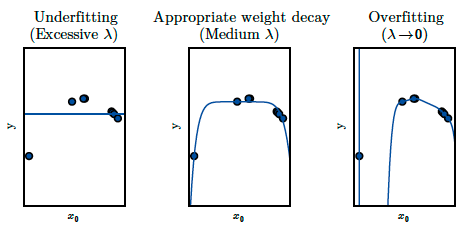
\includegraphics[width=0.99\textwidth]
                {./images/training_issues/goodfellow17_regularisation_weigh_decay_example_1.png}\\
            \vspace{0.0cm}
            {\tiny 
                Using weight decay to control a model's tendency to overfit or underfit.\\
                \color{col:attribution} 
                Schematic reproduced from p. 116 of \cite{Goodfellow:2017MITDL}.\\
            }
        \end{center}        
    \end{column}
    \begin{column}{0.28\textwidth}
        {\scriptsize
        The example on the left, 
        shows the impact of different values of $\lambda$ 
        on the result of training a high-degree (degree 9) 
        polynomial regression model
        to examples from a quadratic data-generating distribution.\\
        }
    \end{column}
\end{columns}

\framebreak

%
%

Several \index{regularisation}\gls{regularisation} 
techniques are known to \gls{ml} practitioners.\\
\vspace{0.3cm}

Broadly speaking, we can distinguish between techniques that:\\
\vspace{0.1cm}
\begin{itemize}
    \item 
    {\bf modify the \index{loss function}\gls{loss function}}
    \begin{itemize}
        \item e.g. L2 \gls{regularisation}, L1 \gls{regularisation}, entropy
    \end{itemize}
    \vspace{0.1cm}
    \item
    {\bf modify the data sampling method}
    \begin{itemize}
        \item e.g. data augmentation, k-fold cross-validation
    \end{itemize}
    \vspace{0.1cm}
    \item
    {\bf modify the training method}
    \begin{itemize}
        \item e.g. noise injection, dropout
    \end{itemize}
\end{itemize}

\vspace{0.3cm}

We will have a closer look at \gls{regularisation} 
techniques later in Part {\thispart}.\\

\end{frame}

\section{Bias-variance trade-off}

\begin{frame}[t]{Point estimation}

    In statistic, 
    \index{point estimation}\gls{point estimation}
    is the {\bf derivation of a best estimate
    for a quantity of interest}, using a sample of data.
    \begin{itemize}
        \item
        Typically, the quantity of interest is a 
        single parameter, or a vector of parameters, 
        controlling a parametric model.
        \item
        To distinguish the estimates of parameters of
        interest from their true or other values,
        we will use $\vect{\hat{\theta}}$ to denote the 
        point estimate of $\vect{\theta}$.
    \end{itemize}

    \vspace{0.1cm}

    If $\mathbb{X}_{m}$ = $\{\vect{x}_{1}, ..., \vect{x}_{m}\}$ is a set
    of $m$ independent and identically distributed (i.i.d.) points,
    a \index{point estimator}\gls{point estimator}\footnote{
        also known as a {\em statistic}} 
    is any function of the data:

    \begin{equation}
        \vect{\hat{\theta}}_{\mathbb{X}_{m}} = g(\vect{x}_{1}, ..., \vect{x}_{m})
        \label{eq:point_estimator}
    \end{equation}\\

    \vspace{0.2cm}
    While any function qualifies as a \gls{point estimator}, 
    a good estimator gets close to the true value of $\vect{\theta}$
    that generated the sample of data.\\

    \vspace{0.2cm}
    Since the data are drawn randomly, 
    $\vect{\hat{\theta}}_{\mathbb{X}_{m}}$ itself is a random variable.\\

\end{frame}

\begin{frame}[t]{Bias}

The \index{bias}\gls{bias} of an estimator is defined as:

\begin{equation}
    bias(\vect{\hat{\theta}}_{\mathbb{X}_{m}}) = 
      \mathbb{E}(\vect{\hat{\theta}}_{\mathbb{X}_{m}}) - \vect{\theta}
    \label{eq:bias}
\end{equation}\\

An estimator is said to be {\bf unbiased} if:
\begin{equation}
    bias(\vect{\hat{\theta}}_{\mathbb{X}_{m}}) = 0
    \label{eq:unbiased_estimator_1}
\end{equation}\\
which implies that:
\begin{equation}
    \mathbb{E}(\vect{\hat{\theta}}_{\mathbb{X}_{m}}) = \vect{\theta}
    \label{eq:unbiased_estimator_2}
\end{equation}\\

An estimator is said to be {\bf asymptotically unbiased} if:
\begin{equation}
    \lim_{m\rightarrow \infty} bias(\vect{\hat{\theta}}_{\mathbb{X}_{m}}) = 0
    \label{eq:asymptotically_unbiased_estimator_1}
\end{equation}\\

While it is desirable to avoid biases, 
unbiased estimators are not always the best estimators to use 
(see later in this lecture).

\end{frame}

\begin{frame}[t,allowframebreaks]{Variance -}

    Another property of an estimator is its \index{variance}\gls{variance}.\\

    \begin{equation}
        var(\vect{\hat{\theta}}_{\mathbb{X}_{m}}) = 
          \mathbb{E}(\vect{\hat{\theta}}_{\mathbb{X}_{m}}) - \vect{\theta}
        \label{eq:variance}
    \end{equation}\\
    
    It is a measure of how much our estimation 
    would vary if repeated with independent data samples from 
    the same data-generating process.

    The square root of \gls{variance} is known as 
    the \index{standard error}\gls{standard error}.

    Ideally, we prefer 

\end{frame}

\begin{frame}[t,allowframebreaks]{
    Bias and variance examples for simple estimators -}


    
\end{frame}


\begin{frame}[t,allowframebreaks]{
    Trade off between bias and variance -}

The \index{bias}\gls{bias} and the \index{variance}\gls{variance}
are {\bf different sources of error} in an estimator.\\
\vspace{0.2cm}

The {\bf mean squared error (MSE) or our estimate},
expressing the overall expected (squared) deviation, 
is given by:
\begin{equation}
    MSE = 
      \mathbb{E}\Big( 
        (\vect{\hat{\theta}}_{\mathbb{X}_{m}} - \vect{\theta})^2        
       \Big) =
       bias(\vect{\hat{\theta}}_{\mathbb{X}_{m}})^2 +
       var(\vect{\hat{\theta}}_{\mathbb{X}_{m}})
    \label{eq:mse_estimation}
\end{equation}\\

\vspace{0.2cm}

{\bf Desirable estimators have small MSE.}
\begin{itemize}
    \item
    Between estimators with more \gls{bias} and estimators 
\end{itemize}

\framebreak

%
%

The relationship between \gls{bias} and \gls{variance} is
linked to the concept of a 
\gls{ml} model \index{capacity}\gls{capacity}
and to the pathologies of 
\index{underfitting}\gls{underfitting} and
\index{overfitting}\gls{overfitting}.

\begin{center}
    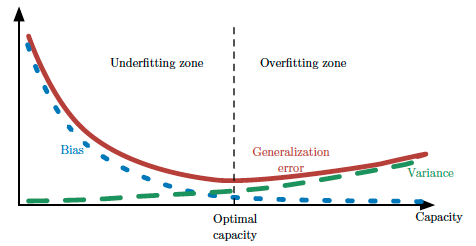
\includegraphics[width=0.80\textwidth]
        {./images/training_issues/goodfellow17_bias_variance_tradeoff_1.png}\\
    {\tiny 
        Illustrating the trade off between bias and variance.
        As the capacity increases, bias decreases and variance increases
        yielding a U-shaped curve from where an optimal capacity can be deduced.\\
        \color{col:attribution} 
        Schematic reproduced from p. 127 of \cite{Goodfellow:2017MITDL}.\\
    }
\end{center}        

\end{frame}


\begin{frame}[t,allowframebreaks]{
    Maximum Likelihood Estimation -}

\end{frame}

\section{Regularisation revisited}
\subsection{Norm penalties: L2 and L1 regularisation}
\subsection{Dataset augmentation}
\subsection{Noise robustness}
\subsection{Multitask learning}
\subsection{Early stopping}
\subsection{Parameter sharing}
\subsection{Ensemble methods: Bagging, subsampling and dropout}
\subsection{Adversarial Training}

% Computation graph introduction and examples
\section{Computation Graph}
%
% The Computation Graph
%

\begin{frame}[t]{The Computation Graph} 

    Any function that can be written down algebraically, 
    can be {\bf decomposed to elementary functions and operations}.\\
    \vspace{0.2cm}
    This {\bf decomposition can be organised in a \gls{computation graph}},
    which allows us to understand the structure of the function and
    to evaluate it in a programmatic way.\\
    \vspace{0.2cm}
    
    \begin{blockexample}{Graphs}
    {\small
    A graph is a network of points (also called graph vertices, or nodes)
    and lines (also called graph edges, or arcs) connecting some subset of points.
    
    There are several types of graphs.
    Here, we will work with simple, labeled, directional graphs:
    \begin{itemize}
        \scriptsize
        \item 
        A simple graph is one where any two points are
        connected, at most, by one line. 
        \item
        A labeled graph is one in which points, lines, or both, are assigned  labels so 
        the carry more information than what is encoded in their intrinsic connectivity.
        \item
        A directed graph is one in which lines have a direction (from a parent to a child node).
    \end{itemize}
    }
    \end{blockexample}
    
\end{frame}

%
% Example computation graph for a simple function R->R
%

\begin{frame}[t,allowframebreaks]{
  Example Computation Graph of function $f: \mathbb{R} \rightarrow \mathbb{R}$ -} 
   
  \vspace{-0.2cm}
  Consider the following example function $f$ of a single argument $w$:\\
  %\vspace{-0.3cm}
  \begin{equation}
    f(w) =  w^2ln(w) + tanh(w)
    \label{eq:computational_graph_example_function_1}
  \end{equation}
  %\vspace{-0.2cm}
  Its computation graph is shown below.\\
  %\vspace{-0.2cm}

  \begin{center}
     \begin{tikzpicture}[scale=0.92]
   
       %\draw[help lines] (0,0) grid (11,6);
       
       \node[input_graph_node]   (w)  at (0.0, 5.0) {$w$};
       \node[general_graph_node] (u1) at (2.6, 5.0) {$()^2$};
       \node[general_graph_node] (u2) at (2.6, 3.0) {$ln$};
       \node[general_graph_node] (u3) at (2.6, 1.0) {\small $tanh$};
       \node[general_graph_node] (u4) at (6.1, 4.0) {$\times$};
       \node[general_graph_node] (u5) at (7.6, 2.0) {$+$};
   
       \drawgraphlinebigarrow (w.east)       
          to node[above, midway]
          {\small $w$}(u1.west) ;
       \drawgraphlinebigarrow (w.south east) 
          to[bend right] node[left]
          {}(u2.west) ;
       \drawgraphlinebigarrow (w.south)      
         to[bend right=40] node[left]
         {}(u3.west) ;
   
       \drawgraphlinebigarrow (u1.east)       
         to[bend left =10] node[above,midway,xshift=-0.5cm,yshift=0.2cm]
         {\small \color{black} $u_1=w^2$}
         (u4.north west) ;
       \drawgraphlinebigarrow (u2.east)       
         to[bend right=10] node[below,midway,xshift=-0.3cm,yshift=-0.2cm]
         {\small \color{black} $u_2=ln(w)$}
         (u4.south west) ;
       \drawgraphlinebigarrow (u3.east) 
         to[looseness=1,bend right=15] node[below,midway,xshift=-0.9cm,yshift=-0.1cm]
         {\small \color{black} $u_3=tanh(w)$}
         (u5.south west) ;
   
       \drawgraphlinebigarrow (u4.east) 
         to[bend left=10] 
         node[above,midway,xshift=0.5cm,yshift=0.4cm]
         {\small \color{black} $u_4=u_1 u_2$}
         (u5.north) ;
   
       \drawinvisiblegraphline (u5.east) 
         to 
         node[above,midway,xshift=-0.3cm] 
         {\small \color{black} $u_5=u_3+u_4$} 
         (11,2);
   
     \end{tikzpicture}
  \end{center}
   
  \framebreak
   
  Note that {\bf each child node is a function of its parent nodes}. However,
  if we unfold the definition of each node, everything is a function of $w$.\\
  \vspace{0.2cm}
  The computation flows forward (the graph is evaluated from left to right),
  and the final node ($u_5$) evaluates the function $f(w)$.\\
  \vspace{-0.3cm}
     
  \begin{center}
     \begin{tikzpicture}[scale=0.92]
   
       %\draw[help lines] (0,0) grid (11,6);
       
       \node[input_graph_node]   (w)  at (0.0, 5.0) {$w$};
       \node[general_graph_node] (u1) at (2.6, 5.0) {$()^2$};
       \node[general_graph_node] (u2) at (2.6, 3.0) {$ln$};
       \node[general_graph_node] (u3) at (2.6, 1.0) {\small $tanh$};
       \node[general_graph_node] (u4) at (6.1, 4.0) {$\times$};
       \node[general_graph_node] (u5) at (7.6, 2.0) {$+$};
   
       \drawgraphlinebigarrow (w.east)       
          to node[above, midway]
          {\small $w=$ \color{magenta} 3}(u1.west) ;
       \drawgraphlinebigarrow (w.south east) 
          to[bend right] node[left]
          {}(u2.west) ;
       \drawgraphlinebigarrow (w.south)      
         to[bend right=40] node[left]
         {}(u3.west) ;
   
       \drawgraphlinebigarrow (u1.east)       
         to[bend left =10] node[above,midway,xshift=-0.2cm,yshift=0.2cm]
         {\small \color{black} $u_1=w^2=$ \color{magenta} 9}
         (u4.north west) ;
       \drawgraphlinebigarrow (u2.east)       
         to[bend right=10] node[below,midway,xshift=0.4cm,yshift=-0.2cm]
         {\small \color{black} $u_2=ln(w)=$ \color{magenta} 1.0986}
         (u4.south west) ;
       \drawgraphlinebigarrow (u3.east) 
         to[looseness=1,bend right=15] node[below,midway,xshift=-0.2cm,yshift=-0.1cm]
         {\small \color{black} $u_3=tanh(w)=$ \color{magenta} 0.9951}
         (u5.south west) ;
   
       \drawgraphlinebigarrow (u4.east) 
         to[bend left=10] 
         node[above,midway,xshift=1.2cm,yshift=0.4cm]
         {\small \color{black} $u_4=u_1 u_2=$ \color{magenta} 9.8874}
         (u5.north) ;
   
       \drawinvisiblegraphline (u5.east) 
         to 
         node[above,midway,xshift=0.6cm] 
         {\small \color{black} $u_5=u_3+u_4=$ \color{magenta} 10.8825} 
         (11,2);
   
     \end{tikzpicture}
  \end{center}
     
\end{frame}
   
%
% Another example computation graph for a simple function R^2->R
%
   
\begin{frame}[t]{
  Example Computation Graph of function $f: \mathbb{R}^2 \rightarrow \mathbb{R}$} 
   
  Similar computation graphs can be constructed for functions 
  that receive multi-dimensional inputs (and/or produce multi-dimensional outputs).\\
  \vspace{0.2cm} 
  A trivial example is shown below for a simple function
  $f: \mathbb{R}^2 \rightarrow \mathbb{R}$:
  \begin{equation}
    f \Big(\mathbf{w}=(w_1,w_2)\Big) =  w_1^2 + w_2^2 
    \label{eq:computational_graph_example_function_2}
  \end{equation}
   
  \begin{center}
     \begin{tikzpicture}[scale=1.0]
       % \draw[help lines] (0,0) grid (11,4);
       
       \node[input_graph_node] (w1) at (0.0, 3.0) {$w_1$};
       \node[input_graph_node] (w2) at (0.0, 1.0) {$w_2$};
   
       \node[general_graph_node] (u1) at (3.0, 3.0) {$()^2$};
       \node[general_graph_node] (u2) at (3.0, 1.0) {$()^2$};
   
       \node[general_graph_node] (u3) at (7.8, 2.0) {$+$};
   
       \drawgraphlinebigarrow (w1.east) 
       to 
       node[above,midway]
       {\scriptsize $w_1$}
       (u1.west) ;
   
       \drawgraphlinebigarrow (w2.east) 
       to 
       node[above,midway]
       {\scriptsize $w_2$}
       (u2.west) ;
   
       \drawgraphlinebigarrow (u1.east) 
       to[bend left =20] 
       node[above,midway,xshift=-0.3cm,yshift=0cm] 
       {\scriptsize $u_1=w_1^2$}
       (u3.north west) ;
   
       \drawgraphlinebigarrow (u2.east) 
       to[bend right=20] 
       node[above,midway,xshift=-0.3cm,yshift=0cm] 
       {\scriptsize $u_2=w_2^2$}
       (u3.south west) ;
   
       \drawinvisiblegraphline (u3.east) 
       to 
       node[above,midway,xshift=0.2cm] 
       {\scriptsize \color{black} $u_3=u_1+u_2$} 
       (10.5,2.0);
   
     \end{tikzpicture}
  \end{center}
   
\end{frame}
   

% Automatic differentiation examples
\section{Automatic Differentiation}
%
% Intro to Automatic Differentiation
%

\begin{frame}[t,allowframebreaks]{Introduction to Automatic Differentiation -} 

  \index{AD}\index{automatic differentiation}\gls{ad} 
  is a technique to {\bf evaluate the derivative
  of a function} specified by a 
  \gls{computation graph}.\\
  \vspace{0.2cm}

  It is also called
  \index{algorithmic differentiation}\gls{algorithmic differentiation}, or
  \index{computational differentiation}\gls{computational differentiation}.\\
  \vspace{0.2cm}

  The technique works by exploiting the function decomposition expressed in the
  computation graph, and {\bf applying the chain rule repeatedly}.\\
  \vspace{0.2cm}
  
  \gls{ad} has a number of advantages:
  \begin{itemize}
    \item It is easily programmable.
    \item It is {\bf efficient}.
    \item It is {\bf numerically stable}.
  \end{itemize}
  
  \framebreak
  
  Note that automatic differentiation {\bf differs from both}:
  \begin{itemize}
    \item {\bf symbolic differentiation}, and
    \item {\bf numerical differentiation}
  \end{itemize}
  
  \begin{blockexample}{Symbolic differentiation}
  \end{blockexample}

  \begin{blockexample}{Numerical differentiation}
  \end{blockexample}

\end{frame}

%
% Automatic Differentiation: How it works
%

\begin{frame}[t,allowframebreaks]{Automatic Differentiation: How it works -} 

  For a given function $f: \mathbb{R}^n \rightarrow \mathbb{R}^m$,
  the corresponding \index{Jacobian matrix}\gls{Jacobian matrix} 
  $\vect{J}_f$ has $m$ rows and $n$ columns.
  Its element at row $i$ and column $j$, is given by:
  
  \begin{equation}
    {J_f}_{ij} = \frac{\partial f_i}{\partial w_j}
    \label{eq:ad_jacobian_element_1}
  \end{equation}
  
  where $f_i$ is the $i^{th}$ element of the function $f=(f_1, f_2, ..., f_m)$,
  and $w_j$ is the $j^{th}$ element of the input vector $\vect{w}=(w_1, w_2, ..., w_n)$.\\
  
  \vspace{0.2cm}
  
  Suppose that the function $f$ is a composite function:
  \begin{equation}
    \vect{f}(\vect{w}) = 
      (\vect{h} \circ \vect{g}) (\vect{w})= \vect{h}(\vect{g}(\vect{w}))
    \label{eq:ad_composite_function_1}
  \end{equation}
  
  with $\vect{w} \in \mathbb{R}^n$, 
  $g: \mathbb{R}^n \rightarrow \mathbb{R}^k$, and
  $h: \mathbb{R}^k \rightarrow \mathbb{R}^m$.
  
  \framebreak
  
  Applying the chain rule, 
  the element at row $i$ and column $j$
  of the $m \times n$ \index{Jacobian matrix}\gls{Jacobian matrix} $\vect{J}$ of 
  the composite function $\vect{f}$ is:
  \begin{equation}
    {J_f}_{ij} = 
      \frac{\partial f_i}{\partial w_j} = 
      \sum_{k} \frac{\partial f_i}{\partial g_k} \frac{\partial g_k}{\partial w_j}
      \label{eq:ad_jacobian_element_composite_function_1}
  \end{equation}
  
  In more compact notation, 
  the \gls{Jacobian matrix} $\vect{J}_{f}$ can be written as:
  \begin{equation}
    J_{f} = J_{h} J_{g}
      \label{eq:ad_jacobian_composite_function_1}
  \end{equation}
  
  More generally, if $\vect{f}$ is a composite of $\ell$ functions $f_1$,...,$f_\ell$:
  \begin{equation}
    \vect{f}(\vect{w}) = 
      (\vect{f_{\ell}} \circ \vect{f_{\ell-1}} \circ ... 
        \circ \vect{f_1})(\vect{w})= \vect{f_{\ell}}(\vect{f_{\ell-1}}(...(\vect{f_1}(\vect{w}))))
    \label{eq:ad_composite_function_2}  
  \end{equation}
  
  the corresponding 
  \index{Jacobian matrix}\gls{Jacobian matrix} $\vect{J}_{f}$ 
  can be written as:
  \begin{equation}
    J_{f} = J_{f_{\ell}} J_{f_{\ell-1}} ... J_{f_1}
    \label{eq:ad_jacobian_composite_function_2}
  \end{equation}
  
  \framebreak
  
  There are two distinct types of automatic differentiation:
  
  \begin{itemize}
    \item 
      Forward mode of automatic differentiation 
      (or forward accumulation).\\
      In this mode, we traverse the chain rule from inside to outside:\\
      First we evaluate $\displaystyle \frac{\partial f_1}{\partial w}$,
      then $\displaystyle \frac{\partial f_2}{\partial f_1}$,
      and at last $\displaystyle \frac{\partial f_\ell}{\partial f_{\ell-1}}$
    \item 
      Reverse mode of automatic differentiation 
      (or reverse accumulation).\\
      In this mode, we traverse the chain rule from outside to inside.
  \end{itemize}
  
  \vspace{0.2cm}
  
  Given a function $f: \mathbb{R}^n \rightarrow \mathbb{R}^m$,
  \begin{itemize}
    \item 
      the forward mode is more efficient if $n << m$, and
    \item 
      the reverse mode is more efficient if $n >> m$.
  \end{itemize}
  
\end{frame}
  
  
%
% Forward Mode of Automatic Differentiation
%

\begin{frame}[t]{Forward Mode of Automatic Differentiation} 

  A decomposition of a function $\vect{f}$ 
  into a \gls{computation graph},
  also allows us to break down the action of the 
  \index{Jacobian matrix}\gls{Jacobian matrix} $\vect{J}_{f}$.\\
  \vspace{0.2cm}
    
  The action of $\vect{J}_{f}$
  can be {\bf evaluated sequentially} 
  using Eq.~\ref{eq:ad_jacobian_composite_function_2}.\\
  \vspace{0.2cm}

  Given a vector $\vect{u}_0$, an iteration of forward \gls{ad}
  numerically evaluates $\vect{J_f} \cdot \vect{u}_0$:\\    
  \vspace{-0.4cm}
  \begin{equation}
    \begin{split}
      \vect{J_f} \cdot \vect{u}_0 
      & = J_{f_{\ell}} \cdot J_{f_{\ell-1}} \cdot ... \cdot J_{f_2} \cdot J_{f_1} \cdot u_0 \\
      & = J_{f_{\ell}} \cdot J_{f_{\ell-1}} \cdot ... \cdot J_{f_2} \cdot u_1 \\
      & = J_{f_{\ell}} \cdot J_{f_{\ell-1}} \cdot ... \cdot u_2 \\
      & = ... \\
      & = J_{f_{\ell}} \cdot u_{\ell-1}  \\
      & = u_{\ell}  \\
    \end{split}
  \end{equation}
    
  where the vectors $\vect{u_k}$ satisfy the recursive relationship:\\
  \vspace{-0.3cm}
  \begin{equation}
    u_k = J_k u_{k-1} %\textrm{, for } k=1,...,\ell
  \end{equation}
    
\end{frame}
  
%
% Reverse Mode of Automatic Differentiation
%

\begin{frame}[t]{Reverse Mode of Automatic Differentiation} 

\end{frame}


%
%
%

\begin{frame}[t,allowframebreaks]{
    Example / Forward Mode of Automatic Differentiation -} 
   
  \vspace{-0.2cm}
  We have studied the computation graph of the function 
  $f: \mathbb{R} \rightarrow \mathbb{R}$ given 
  in Eq.~\ref{eq:computational_graph_example_function_1}.
  We will use that graph to evaluate the derivative $df/dw$.\\
   
  % Show the computation graph again and highlight derivatives at each node
  %
   
  \begin{center}
    \begin{tikzpicture}[scale=0.90]
   
       %\draw[help lines] (0,0) grid (11,6);
       
       \node[input_graph_node]   (w)  at (0.0, 5.0) {$w$};
       \node[general_graph_node] (u1) at (2.6, 5.0) {$()^2$};
       \node[general_graph_node] (u2) at (2.6, 3.0) {$ln$};
       \node[general_graph_node] (u3) at (2.6, 1.0) {\small $tanh$};
       \node[general_graph_node] (u4) at (6.1, 4.0) {$\times$};
       \node[general_graph_node] (u5) at (7.6, 2.0) {$+$};
   
       \drawgraphlinebigarrow (w.east)       
          to node[above, midway]
          {\small \color{black} $w$, 
            \color{red} $\displaystyle \frac{dw}{dw}$}(u1.west) ;
       \drawgraphlinebigarrow (w.south east) 
          to[bend right] node[left]
          {}(u2.west) ;
       \drawgraphlinebigarrow (w.south)      
         to[bend right=40] node[left]
         {}(u3.west) ;
   
       \drawgraphlinebigarrow (u1.east)       
         to[bend left =10] node[above,midway,xshift=-0.3cm,yshift=0.2cm]
         {\small \color{black} $u_1=w^2$, 
           \color{red} $\displaystyle \frac{du_1}{dw}$}
         (u4.north west) ;
       \drawgraphlinebigarrow (u2.east)       
         to[bend right=10] node[below,midway,xshift=-0.1cm,yshift=-0.2cm]
         {\small \color{black} $u_2=ln(w)$,
           \color{red} $\displaystyle \frac{du_2}{dw}$}
         (u4.south west) ;
       \drawgraphlinebigarrow (u3.east) 
         to[looseness=1,bend right=15] node[below,midway,xshift=-0.7cm,yshift=-0.1cm]
         {\small \color{black} $u_3=tanh(w)$,
           \color{red} $\displaystyle \frac{du_3}{dw}$}
         (u5.south west) ;
   
       \drawgraphlinebigarrow (u4.east) 
         to[bend left=10] 
         node[above,midway,xshift=0.7cm,yshift=0.4cm]
         {\small \color{black} $u_4=u_1 u_2$,
           \color{red} $\displaystyle \frac{du_4}{dw}$}
         (u5.north) ;
   
       \drawinvisiblegraphline (u5.east) 
         to 
         node[above,midway,xshift=0.0cm] 
         {\small \color{black} $u_5=u_3+u_4$,
           \color{red} $\displaystyle \frac{du_5}{dw}$} 
         (11,2);
   
    \end{tikzpicture}
  \end{center}
   
  \framebreak
   
  % List the derivatives of u1,...,u5
  %
   
  \vspace{-0.1cm}
   
  \begin{equation}
    \frac{d u_1}{d w} =  
    \frac{d}{dw} \Big(w^2\Big) = 2w
  \end{equation}
   
  \vspace{-0.1cm}
   
  \begin{equation}
    \frac{du_2}{dw} =  
    \frac{d}{dw} \Big( ln(w) \Big) = \frac{1}{w}
  \end{equation}
   
  \vspace{-0.1cm}
   
  \begin{equation}
    \frac{du_3}{dw} =  
    \frac{d}{dw} \Big( tanh(w) \Big) = 1-tanh^2(w)
  \end{equation}
   
  \vspace{-0.1cm}
   
  \begin{equation}
    \frac{du_4}{dw} =  
      \frac{d}{dw} \Big( u_1 u_2 \Big) = 
      2w ln(w) + w
  \end{equation}
   
  \vspace{-0.3cm}
   
  \begin{equation}
    \frac{du_5}{dw} =  
      \frac{d}{dw} \Big( u_3 + u_4 \Big) = 
      \frac{du_3}{dw} + \frac{du_4}{dw} =
      1-tanh^2(w) + 2w ln(w) + w
  \end{equation}
   
  \framebreak
   
  \begin{center}
    \begin{tikzpicture}
   
       %\draw[help lines] (0,0) grid (11,6);
       
       \node[input_graph_node]   (w)  at (0.0, 5.0) {$w$};
       \node[general_graph_node] (u1) at (2.6, 5.0) {$()^2$};
       \node[general_graph_node] (u2) at (2.6, 3.0) {$ln$};
       \node[general_graph_node] (u3) at (2.6, 1.0) {\small $tanh$};
       \node[general_graph_node] (u4) at (6.1, 4.0) {$\times$};
       \node[general_graph_node] (u5) at (7.6, 2.0) {$+$};
   
       \drawgraphlinebigarrow (w.east)       
          to node[above, midway]
          {\small $\color{black} w, 
           \color{red} \cancelto{1}{\displaystyle \frac{dw}{dw}}$}(u1.west) ;
       \drawgraphlinebigarrow (w.south east) 
          to[bend right] node[left]
          {}(u2.west) ;
       \drawgraphlinebigarrow (w.south)      
         to[bend right=40] node[left]
         {}(u3.west) ;
   
       \drawgraphlinebigarrow (u1.east)       
         to[bend left =10] node[above,midway,xshift=0.4cm]
         {\small $\color{black} u_1=w^2, 
           \color{red} \displaystyle \frac{du_1}{dw}=2w$}
         (u4.north west) ;
       \drawgraphlinebigarrow (u2.east)       
         to[bend right=10] node[below,midway,xshift=0.4cm]
         {\small $\color{black} u_2=ln(w), 
           \color{red} \displaystyle \frac{du_2}{dw}=\frac{1}{w}$}
         (u4.south west) ;
   
       \drawgraphlinebigarrow (u3.east) 
         to[looseness=1,bend right=15] node[below,midway,xshift=0.6cm]
         {\small $\color{black} u_3=tanh(w), 
           \color{red} \displaystyle \frac{du_3}{dw}=1-tanh^2(w)$}
         (u5.south west) ;
   
       \drawgraphlinebigarrow (u4.east) 
         to[bend left=10] 
         node[above,midway,xshift=0.9cm,yshift=1cm]
         {\small \color{black} $u_4=u_1 u_2$}
         node[below,midway,xshift=1.8cm,yshift=1cm]
         {\small \color{red} 
           $\displaystyle \frac{du_4}{dw}=\frac{du_1}{dw}u_2+u_1\frac{du_2}{dw}$}
         (u5.north) ;
   
       \drawinvisiblegraphline (u5.east) 
         to 
         node[above,midway,xshift=0.0cm] 
         {\small \color{black} $u_5=u_3+u_4$} 
         node[below,midway,xshift=0.0cm] 
         {\small \color{red} 
           $\displaystyle \frac{du_5}{dw}=\frac{du_3}{dw}+\frac{du_4}{dw}$} 
         (11,2);
   
     \end{tikzpicture}
  \end{center}

\end{frame}
   
%
% Discuss inefficiencies of the Forward Mode for graphs with more sparse
% connections, leading up to illustrations of the Reverse Mode
%

\begin{frame}[t,allowframebreaks]{
    Differentiation of functions of multidimensional input -} 
   
  \vspace{-0.2cm}
  We can use the previous ideas of Forward Mode Automatic Differentiation for functions
  of multidimensional variables $\vect{w} \in \mathbb{R}^n$.\\
  This requires the evaluation of the full gradient $\nabla_{w}u$ at each node $u$.\\
   
  % Show a generic fully connected graph
  %
  \begin{center}
     \begin{tikzpicture}[scale=0.9]
   
       %\draw[help lines] (0,0) grid (11,6);
       
       \node[input_graph_node] (w1) at (0.0, 5.6) {$w_1$};
       \node[input_graph_node] (w2) at (0.0, 3.9) {$w_2$};
       \node[input_graph_node] (w3) at (0.0, 2.2) {$...$};
       \node[input_graph_node] (wn) at (0.0, 0.5) {$w_n$};
   
       \node[general_graph_node] (u11) at (4.0, 5.15) {$u^1_1$};
       \node[general_graph_node] (u12) at (4.0, 3.70) {$u^1_2$};
       \node[general_graph_node] (u13) at (4.0, 2.25) {$...$};
       \node[general_graph_node] (u1m) at (4.0, 0.80) {$u^1_m$};
   
       \node[general_graph_node] (u21) at (7.8, 5.0) {$u^2_1$};
       \node[general_graph_node] (u22) at (7.8, 3.0) {$...$};
       \node[general_graph_node] (u2l) at (7.8, 1.0) {$u^2_\ell$};
   
       \node[general_graph_node] (u31) at (10.0, 4.0) {$...$};
       \node[general_graph_node] (u32) at (10.0, 2.0) {$...$};
   
       \drawgraphlinebigarrow       (w1.east) to node[above,midway]
          {$w_1, \color{red} \displaystyle \nabla_{\bf{w}}w_1$}(u11.west) ;
       \drawgraphlinebigarrow       (w1.east) to node{} (u12.west) ;
       \drawgraphdashedlinebigarrow (w1.east) to node{} (u13.west) ;
       \drawgraphlinebigarrow       (w1.east) to node{} (u1m.west) ;
   
       \drawgraphlinebigarrow       (w2.east) to node{} (u11.west) ;
       \drawgraphlinebigarrow       (w2.east) to node{} (u12.west) ;
       \drawgraphdashedlinebigarrow (w2.east) to node{} (u13.west) ;
       \drawgraphlinebigarrow       (w2.east) to node{} (u1m.west) ;
   
       \drawgraphdashedlinebigarrow (w3.east) to node{} (u11.west) ;
       \drawgraphdashedlinebigarrow (w3.east) to node{} (u12.west) ;
       \drawgraphdashedlinebigarrow (w3.east) to node{} (u13.west) ;
       \drawgraphdashedlinebigarrow (w3.east) to node{} (u1m.west) ;    
       
       \drawgraphlinebigarrow       (wn.east) to node{} (u11.west) ;
       \drawgraphlinebigarrow       (wn.east) to node{} (u12.west) ;
       \drawgraphdashedlinebigarrow (wn.east) to node{} (u13.west) ;
       \drawgraphlinebigarrow       (wn.east) to node[below,midway]
         {$w_n, \color{red} \displaystyle \nabla_{\bf{w}}w_n$} (u1m.west) ;
   
       \drawgraphlinebigarrow (u11.east) 
       to node[above,midway] 
       {\small $u^1_1(\mathbf{w}),
         \color{red} \displaystyle \nabla_{\bf{w}}u^1_1(\mathbf{w})$}(u21.west) ;
       \drawgraphdashedlinebigarrow (u11.east) 
       to node{}(u22.west) ;
       \drawgraphlinebigarrow (u11.east) 
       to node{}(u2l.west) ;
   
       \drawgraphlinebigarrow (u12.east) 
       to node{}(u21.west) ;
       \drawgraphdashedlinebigarrow (u12.east) 
       to node{}(u22.west) ;
       \drawgraphlinebigarrow (u12.east) 
       to node{}(u2l.west) ;
   
       \drawgraphdashedlinebigarrow (u13.east) 
       to node{}(u21.west) ;
       \drawgraphdashedlinebigarrow (u13.east) 
       to node{}(u22.west) ;
       \drawgraphdashedlinebigarrow (u13.east) 
       to node{}(u2l.west) ;
   
       \drawgraphlinebigarrow (u1m.east) 
       to node{}(u21.west) ;
       \drawgraphdashedlinebigarrow (u1m.east) 
       to node{}(u22.west) ;
       \drawgraphlinebigarrow (u1m.east) 
       to node[below,midway,yshift=-0.1cm]
       {\small $u^1_m(\mathbf{w}),
         \color{red} \displaystyle \nabla_{\bf{w}}u^1_m(\mathbf{w})$}(u2l.west) ;
   
       \drawgraphdashedlinebigarrow (u21.east) 
       to node[above,midway,xshift=1.2cm]
       {\small $u^2_1(\mathbf{u}^1),
         \color{red} \displaystyle \nabla_{\bf{w}}u^2_1(\mathbf{u}^1)$}(u31.west) ;
       \drawgraphdashedlinebigarrow (u21.east) 
       to node{}(u32.west) ;
   
       \drawgraphdashedlinebigarrow (u22.east) 
       to node{}(u31.west) ;
       \drawgraphdashedlinebigarrow (u22.east) 
       to node{}(u32.west) ;
   
       \drawgraphdashedlinebigarrow (u2l.east) 
       to node{}(u31.west) ;
       \drawgraphdashedlinebigarrow (u2l.east) 
       to node[below,midway,xshift=1.2cm]
       {\small $u^2_\ell(\mathbf{u}^1),
         \color{red} \displaystyle \nabla_{\bf{w}}u^2_\ell(\mathbf{u}^1)$}(u32.west) ;
   
     \end{tikzpicture}
  \end{center}
   
  \framebreak
   
  % Illustrate repeated computation of derivatives known to be 0
  %
     
  The Forward Mode can be inefficient for graphs 
  where the inputs have sparse connectivity.
  Calculation of the complete gradient at each node, 
  can lead to repeated computation of derivatives known to be 0.\\
  Consider the following simple function and its corresponding graph:\\
  \begin{equation}
    f\Big(\mathbf{w}=(w_1,w_2)\Big) =  w_1^2 + w_2^2 
    \label{eq:ad_example_multidim_function_1}
  \end{equation}
   
  % Show an example with a function of a 2-dimensional input
  %
  \begin{center}
     \begin{tikzpicture}[scale=0.98]
   
       % \draw[help lines] (0,0) grid (11,4);
       
       \node[input_graph_node] (w1) at (0.0, 3.0) {$w_1$};
       \node[input_graph_node] (w2) at (0.0, 1.0) {$w_2$};
   
       \node[general_graph_node] (u1) at (3.0, 3.0) {$()^2$};
       \node[general_graph_node] (u2) at (3.0, 1.0) {$()^2$};
   
       \node[general_graph_node] (u3) at (7.8, 2.0) {$+$};
   
       \drawgraphlinebigarrow (w1.east) 
       to 
       node[above,midway]
       {\scriptsize $w_1$}
       node[below,midway]
       {\scriptsize \color{red} $\displaystyle \nabla_{\bf{w}}w_1=(1,0)$}
       (u1.west) ;
   
       \drawgraphlinebigarrow (w2.east) 
       to 
       node[above,midway]
       {\scriptsize $w_2$}
       node[below,midway]
       {\scriptsize \color{red} $\displaystyle \nabla_{\bf{w}}w_2=(0,1)$}
       (u2.west) ;
   
       \drawgraphlinebigarrow (u1.east) 
       to[bend left =20] 
       node[above,midway,xshift=-0.3cm,yshift=0cm] 
       {\scriptsize $u_1=w_1^2$}
       node[below,midway,xshift=-0.3cm,yshift=-0.2cm] 
       {\scriptsize \color{red} 
         $\displaystyle \nabla_{\bf{w}}u_1=(\frac{\partial u_1}{\partial w_1},0)=(2w_1,0)$}
       (u3.north west) ;
   
       \drawgraphlinebigarrow (u2.east) 
       to[bend right=20] 
       node[above,midway,xshift=-0.3cm,yshift=0cm] 
       {\scriptsize $u_2=w_2^2$}
       node[below,midway,xshift=-0.3cm,yshift=-0.2cm] 
       {\scriptsize \color{red} 
         $\displaystyle \nabla_{\bf{w}}u_2=(0,\frac{\partial u_2}{\partial w_2})=(0,2w_2)$}
       (u3.south west) ;
   
       \drawinvisiblegraphline (u3.east) 
       to 
       node[above,midway,xshift=0.0cm] 
       {\scriptsize \color{black} 
         $u_3=u_1+u_2$} 
       node[below,midway,xshift=0.0cm,yshift=0.0cm] 
       {\scriptsize \color{red} 
         $\displaystyle \nabla_{\bf{w}}u_3=\nabla_{\bf{w}}u_1+\nabla_{\bf{w}}u_2$} 
       node[below,midway,xshift=0.1cm,yshift=-0.4cm] 
       {\scriptsize \color{red} 
         $\displaystyle =2(w_1,w_2)$} 
       (11.5,2.0);
   
     \end{tikzpicture}
  \end{center}
   
  \framebreak
   
  % Show an example where the problem is more severe
  %
     
  The number of 0's grows fast as the dimensionality of the input increases.
  Consider the following example:\\
  \vspace{-0.4cm}  
  \begin{equation}
    f\Big(\mathbf{w}=(w_1,w_2,w_3,w_4)\Big) =  w_1^2 + w_2^2 + w_3^2 + w_4^2 
    \label{eq:ad_example_multidim_function_2}
  \end{equation}
   
  \vspace{-0.5cm}
     
  % Another example with a function of a 4-dimensional input
  %
  \begin{center}
     \begin{tikzpicture}[scale=0.95]
   
       %\draw[help lines] (0,0) grid (11,6);
       
       \node[input_graph_node] (w1) at (0.0, 5.0) {$w_1$};
       \node[input_graph_node] (w2) at (0.0, 3.5) {$w_2$};
       \node[input_graph_node] (w3) at (0.0, 2.0) {$w_3$};
       \node[input_graph_node] (w4) at (0.0, 0.5) {$w_4$};
   
       \node[general_graph_node] (u1) at (3.6, 5.0) {$()^2$};
       \node[general_graph_node] (u2) at (3.6, 3.5) {$()^2$};
       \node[general_graph_node] (u3) at (3.6, 2.0) {$()^2$};
       \node[general_graph_node] (u4) at (3.6, 0.5) {$()^2$};
   
       \node[general_graph_node] (u5) at (6.7, 4.25) {$+$};
       \node[general_graph_node] (u6) at (6.7, 1.25) {$+$};
   
       \node[general_graph_node] (u7) at (8.7, 2.75) {$+$};
   
       \drawgraphlinebigarrow (w1.east) 
       to 
       node[above,midway]
       {\scriptsize $w_1$}
       node[below,midway]
       {\scriptsize \color{red} $\displaystyle \nabla_{\bf{w}}w_1=(1,0,0,0)$}
       (u1.west) ;
   
       \drawgraphlinebigarrow (w2.east) 
       to 
       node[above,midway]
       {\scriptsize $w_4$}
       node[below,midway]
       {\scriptsize \color{red} $\displaystyle \nabla_{\bf{w}}w_2=(0,1,0,0)$}
       (u2.west) ;
   
       \drawgraphlinebigarrow (w3.east) 
       to 
       node[above,midway]
       {\scriptsize $w_3$}
       node[below,midway]
       {\scriptsize \color{red} $\displaystyle \nabla_{\bf{w}}w_3=(0,0,1,0)$}
       (u3.west) ;
   
       \drawgraphlinebigarrow (w4.east) 
       to 
       node[above,midway]
       {\scriptsize $w_4$}
       node[below,midway]
       {\scriptsize \color{red} $\displaystyle \nabla_{\bf{w}}w_4=(0,0,0,1)$}
       (u4.west) ;
   
       \drawgraphlinebigarrow (u1.east) 
       to[bend left =20] 
       node[above,midway,xshift=0.9cm] 
       {\scriptsize $u_1=w_1^2, \color{red} \displaystyle \nabla_{\bf{w}}u_3=(2w_1,0,0,0)$}
       (u5.north west) ;
   
       \drawgraphlinebigarrow (u2.east) 
       to[bend right=20] 
       node[below,midway,xshift=0.9cm] 
       {\scriptsize $u_2=w_2^2, \color{red} \displaystyle \nabla_{\bf{w}}u_4=(0,2w_2,0,0)$}
       (u5.south west) ;
   
       \drawgraphlinebigarrow (u3.east) 
       to[bend left =20] 
       node[above,midway,xshift=0.9cm] 
       {\scriptsize $u_3=w_3^2, \color{red} \displaystyle \nabla_{\bf{w}}u_3=(0,0,2w_3,0)$}
       (u6.north west) ;
   
       \drawgraphlinebigarrow (u4.east) 
       to[bend right=20] 
       node[below,midway,xshift=0.9cm] 
       {\scriptsize $u_4=w_4^2, \color{red} \displaystyle \nabla_{\bf{w}}u_4=(0,0,0,2w_4)$}
       (u6.south west) ;
   
       \drawgraphlinebigarrow (u5.east) 
       to[bend left =20] 
       node[above,midway,xshift=0.8cm,yshift=0.3cm] 
       {\scriptsize $u_5=u_1+u_2$}
       node[above,midway,xshift=1.5cm,yshift=-0.1cm] 
       {\scriptsize \color{red} 
         $\displaystyle \nabla_{\bf{w}}u_5=\nabla_{\bf{w}}u_1+\nabla_{\bf{w}}u_2$}
       node[above,midway,xshift=1.9cm,yshift=-0.5cm] 
       {\scriptsize \color{red} 
         $\displaystyle =2(w_1,w_2,0,0)$}
       (u7.north) ;
   
       \drawgraphlinebigarrow (u6.east) 
       to[bend right=20]
       node[below,midway,xshift=0.8cm,yshift=0.0cm] 
       {\scriptsize $u_6=u_3+u_4$}
       node[below,midway,xshift=1.5cm,yshift=-0.4cm] 
       {\scriptsize \color{red} 
         $\displaystyle \nabla_{\bf{w}}u_6=\nabla_{\bf{w}}u_3+\nabla_{\bf{w}}u_4$}
       node[below,midway,xshift=1.9cm,yshift=-0.8cm] 
       {\scriptsize \color{red} 
         $\displaystyle =2(0,0,w_3,w_4)$}
       (u7.south) ;
   
       \drawinvisiblegraphline (u7.east) 
       to 
       node[above,midway,xshift=0.0cm] 
       {\scriptsize \color{black} $u_7=u_5+u_6$} 
       node[below,midway,xshift=-0.3cm,yshift=-0.0cm] 
       {\scriptsize \color{red} 
         $\displaystyle \nabla_{\bf{w}}u_7=$}
       node[below,midway,xshift=0.4cm,yshift=-0.4cm] 
       {\scriptsize \color{red} 
         $\displaystyle \nabla_{\bf{w}}u_5+\nabla_{\bf{w}}u_6=$}
       node[below,midway,xshift=0.4cm,yshift=-0.8cm] 
       {\scriptsize \color{red} 
         $\displaystyle 2(w_1,w_2,w_3,w_4)$}
       (11.0,2.75);
   
     \end{tikzpicture}
  \end{center}
   
\end{frame}
   
%
%
%

\begin{frame}[t,allowframebreaks]{
    Reverse Mode of Automatic Differentiation: Example} 

    %
    % forward
    %

    Forward phase:
    
    \begin{center}
        \begin{tikzpicture}[scale=1.0]
    
        % \draw[help lines] (0,0) grid (11,4);
        
        \node[input_graph_node] (w1) at (0.0, 4.0) {$w_1$};
        \node[input_graph_node] (w2) at (0.0, 1.0) {$w_2$};
    
        \node[general_graph_node] (u1) at (5.3, 4.0) {$()^2$};
        \node[general_graph_node] (u2) at (5.3, 1.0) {$()^2$};
    
        \node[general_graph_node] (u3) at (9.0, 2.5) {$+$};
    
        \drawgraphlinebigarrow (w1.east) 
        to 
        node[above,midway]
        {\scriptsize $w_1$}
        node[below,midway]
        {\scriptsize \color{blue} 
         $\displaystyle \frac{\partial w_1}{\partial w_1} = 1$}
        (u1.west) ;
    
        \drawgraphlinebigarrow (w2.east) 
        to 
        node[above,midway]
        {\scriptsize $w_2$}
        node[below,midway]
        {\scriptsize \color{blue} 
          $\displaystyle \frac{\partial w_2}{\partial w_2} = 1$}
        (u2.west) ;
    
        \drawgraphlinebigarrow (u1.east) 
        to[bend left =20] 
        node[above,midway,xshift=-0.3cm,yshift=0cm] 
        {\scriptsize $u_1=w_1^2$}
        node[below,midway,xshift=-0.3cm,yshift=-0.2cm] 
        {\scriptsize \color{green} 
          $\displaystyle \frac{\partial u_1}{\partial w_1}=2w_1$}
        (u3.north west) ;
    
        \drawgraphlinebigarrow (u2.east) 
        to[bend right=20] 
        node[above,midway,xshift=-0.3cm,yshift=0cm] 
        {\scriptsize $u_2=w_2^2$}
        node[below,midway,xshift=-0.3cm,yshift=-0.2cm] 
        {\scriptsize \color{green} 
          $\displaystyle \frac{\partial u_2}{\partial w_2}=2w_2$}
        (u3.south west) ;
    
        \drawinvisiblegraphline (u3.east) 
        to 
        node[above,midway,xshift=0.0cm] 
        {\scriptsize \color{black} $u_3=u_1+u_2$} 
        node[below,midway,xshift=0.0cm,yshift=0.0cm] 
        {\scriptsize \color{red} 
          $\displaystyle \frac{\partial u_3}{\partial u_1}=1,
            \frac{\partial u_3}{\partial u_2}=1$} 
        (11.5,1.8);
    
        \end{tikzpicture}
    \end{center}

    \framebreak
    
    %
    % backward
    %
    
    Backward phase:\\
    
    \begin{center}
        \begin{tikzpicture}[scale=1.0]
    
        % \draw[help lines] (0,0) grid (11,4);
        
        \node[input_graph_node] (w1) at (0.0, 4.0) {$w_1$};
        \node[input_graph_node] (w2) at (0.0, 1.0) {$w_2$};
    
        \node[general_graph_node] (u1) at (5.3, 4.0) {$()^2$};
        \node[general_graph_node] (u2) at (5.3, 1.0) {$()^2$};
    
        \node[general_graph_node] (u3) at (9.0, 2.5) {$+$};
    
        \drawgraphlinebigarrow (w1.east) 
        to 
        node[above,midway]
        {\scriptsize $w_1$}
        node[below,midway]
        {\scriptsize 
         \color{blue}  $\displaystyle \frac{\partial w_1}{\partial w_1}$
         \color{green} $\displaystyle \frac{\partial u_1}{\partial w_1}$
         \color{red}   $\displaystyle \frac{\partial u_3}{\partial u_1}$
         \color{black} $=$ 
         \color{blue}  $(1)$
         \color{green} $(2w_1)$
         \color{red}   $(1)$
        }
        (u1.west) ;
    
        \drawgraphlinebigarrow (w2.east) 
        to 
        node[above,midway]
        {\scriptsize $w_2$}
        node[below,midway]
        {\scriptsize 
         \color{blue}  $\displaystyle \frac{\partial w_2}{\partial w_2}$
         \color{green} $\displaystyle \frac{\partial u_2}{\partial w_2}$
         \color{red}   $\displaystyle \frac{\partial u_3}{\partial u_2}$
         \color{black} $=$ 
         \color{blue}  $(1)$
         \color{green} $(2w_2)$
         \color{red}   $(1)$
        }
        (u2.west) ;
    
        \drawgraphlinebigarrow (u1.east) 
        to[bend left =20] 
        node[above,midway,xshift=-0.3cm,yshift=0cm] 
        {\scriptsize $u_1=w_1^2$}
        node[below,midway,xshift=-0.3cm,yshift=-0.2cm] 
        {\scriptsize 
         \color{green} $\displaystyle \frac{\partial u_1}{\partial w_1}$
         \color{red} $\displaystyle \frac{\partial u_3}{\partial u_1}$
         \color{black} $=$ 
         \color{green} $2w_1$
         \color{red} $1$
        }
        (u3.north west) ;
    
        \drawgraphlinebigarrow (u2.east) 
        to[bend right=20] 
        node[above,midway,xshift=-0.3cm,yshift=0cm] 
        {\scriptsize $u_2=w_2^2$}
        node[below,midway,xshift=-0.3cm,yshift=-0.2cm] 
        {\scriptsize 
         \color{green} $\displaystyle \frac{\partial u_2}{\partial w_2}$
         \color{red} $\displaystyle \frac{\partial u_3}{\partial u_2}$
         \color{black} $=$ 
         \color{green} $2w_2$
         \color{red} $1$
        }
        (u3.south west) ;
    
        \drawinvisiblegraphline (u3.east) 
        to 
        node[above,midway,xshift=0.0cm] 
        {\scriptsize \color{black} $u_3=u_1+u_2$} 
        node[below,midway,xshift=0.0cm,yshift=0.0cm] 
        {\scriptsize \color{red} 
          $\displaystyle 
           \frac{\partial u_3}{\partial u_1}=1,
           \frac{\partial u_3}{\partial u_2}=1$} 
        (11.5,1.8);
    
        \end{tikzpicture}
    \end{center}
    
\end{frame}
    

% Backpropagation
\section{Backpropagation}

% Suggested reading for this part
\section{Suggested reading}
%
%
%

\begin{frame}{Suggested reading for Part \thispart}

    {
        \small
        Essential reading on {\bf automatic differentiation}:
        \begin{itemize}
            \scriptsize
            \item Section 6.5 from the `Deep Learning' 
            textbook of Goodfellow, Bengio and Courville \cite{Goodfellow:2017MITDL}.
            \item Appendix B from the `Machine Learning Refined' 
            textbook of Watt, Borhani and Katsaggelos \cite{Watt:2016Cambridge}.
            \item `A review of automatic differentiation and its 
            efficient implementation' by Margossian \cite{Margossian:2019ad}
        \end{itemize}
        
        Also, you may want to browse:
        \begin{itemize}
            \scriptsize
            \item The collection of articles
             in the book `Automatic Differentiation: Applications, Theory, and Implementations'
             edited by B{\"u}cker, Corliss, Hovland, Naumann and Norris \cite{Bucker:2005ABo}
        \end{itemize}
    }
    

\end{frame}
